%%%%%%%%%%%%%%%%%%%%%%%%%%%%%%%%%%%%%%%%%%%%%%%%%%%%%%%
%% Bachelor's & Master's Thesis Template             %%
%% Copyleft by Artur M. Brodzki & Piotr Woźniak      %%
%% Faculty of Electronics and Information Technology %%
%% Warsaw University of Technology, 2019-2020        %%
%%%%%%%%%%%%%%%%%%%%%%%%%%%%%%%%%%%%%%%%%%%%%%%%%%%%%%%

\documentclass[
    left=2.5cm,         % Sadly, generic margin parameter
    right=2.5cm,        % doesnt't work, as it is
    top=2.5cm,          % superseded by more specific
    bottom=3cm,         % left...bottom parameters.
    bindingoffset=6mm,  % Optional binding offset.
    nohyphenation=false % You may turn off hyphenation, if don't like.
]{template/eiti-thesis}

\addbibresource{ref.bib} % Plik .bib z bibliografią

\begin{document}

%--------------------------------------
% Strona tytułowa
%--------------------------------------
\instytut{Telekomunikacji}
\kierunek{Cyberbezpieczeństwo}
\title{Wybrane metody przeprowadzania i detekcji OSINT}
\engtitle{Selected methods of conducting and detecting OSINT}
\author{tulski}
\album{304217}
\promotor{dr inż. Mariusz Sepczuk}
\date{\the\year}
\maketitle

%--------------------------------------
% Streszczenie po polsku
%--------------------------------------
\newpage %\cleardoublepage % Zaczynamy od nieparzystej strony
\streszczenie \todo{ \lipsum[1] }
\slowakluczowe XXX, XXX, XXX

%--------------------------------------
% Streszczenie po angielsku
%--------------------------------------
\newpage
\abstract \todo{ \lipsum[1] }
\keywords XXX, XXX, XXX

%--------------------------------------
% Oświadczenie o autorstwie
%--------------------------------------
\newpage %\cleardoublepage  % Zaczynamy od nieparzystej strony
\makeauthorship

%--------------------------------------
% Spis treści
%--------------------------------------
\newpage %\cleardoublepage % Zaczynamy od nieparzystej strony

\section*{\contentsname}

\startcontents[mainsections]
\printcontents[mainsections]{l}{1}{\setcounter{tocdepth}{3}}

%--------------------------------------
% Rozdziały
%--------------------------------------
%\cleardoublepage % Zaczynamy od nieparzystej strony
\pagestyle{headings}
\newpage

\section{Teoria związana z tematem pracy}\label{sec:teoria}

\subsection{OSINT}\label{subsec:osint}

\todo{OSINT}

\subsection{Scraping}\label{subsec:scraping}

\todo{Scraping}

\subsection{Web Scraping}\label{subsec:web-scraping}

\todo{Web Scraping}
\newpage

\section{Wykorzystane narzędzia}\label{sec:wykorzystane-narzedzia}

\todo{Ten rodział jest o narzędziach - o czym innym miałby być?}

\subsection{Docker}\label{subsec:docker}

Docker \todo{to narzędzie do... konteneryzacji?}
Opisywana w pracy platforma wykorzystuje technologię konteneryzacji oferowaną przez Docker.

\subsection{Kubernetes}\label{subsec:kubernetes}

\todo{Kubernetes to narzędzie do...}

\subsection{Helm}\label{subsec:helm}

Helm to narzędzie będące menadżerem pakietów w środowisku Kubernetes.
Narzędzie znacznie ułatwia proces wdrażania i utrzymywania aplikacji, szczególnie jeśli są one skomplikowane i złożone z kilku elementów.

\subsection{MicroK8s}\label{subsec:microk8s}

Kubernetes stał się niejako standardem w branży IT\@.
Wraz z wzrostem jego popularności, kolejne osoby oraz firmy zaczęły dostosowywać oryginalny projekt do swoich potrzeb, tym samym tworząc jego własne dystrybucje.
Chociaż wszystkie te dystrybucje mają wspólny fundament, jakim jest oryginalny projekt Kubernetes, każda z nich wnosi unikalne funkcje, narzędzia i optymalizacje.
Przykładowo, dystrybucje takie jak Amazon Elastic Kubernetes Service (Amazon EKS), Google Kubernetes Engine (GKE) czy Azure Kubernetes Service (AKS) zostały specjalnie dostosowane pod specyficzne środowisko chmury poszczególnych dostawcy.

Niniejsza praca wykorzystuje dystrybucję MicroK8s\cite{microk8s-docs-home} ze względu na:
\begin{enumerate}
    \item łatwość instalacji i uruchomienia,
    \item fakt, że jest to lekka dystrybucja K8s, co przekłada się na mniejsze wymagania sprzętowe oraz mniejsze zużycie zasobów,
    \item stabilność - dystrybucja jest przygotowania do produkcyjnego uruchomienia,
    \item prostotę zarządzania - MicroK8s udostępnia rozbudowany interfejs wiersza poleceń (ang. \emph{command line interface, CLI}) ułatwiający konfigurację i utrzymanie środowiska.
\end{enumerate}

\subsection{Medusa}\label{subsec:medusa}

Handel, w tym ten internetowy, jest obecny w naszym życiu od dekad.
Przez swoją bogatą historię stał się jedną z najlepiej opisanych i najbardziej dojrzałych domen.
Większość wyzwań i problemów, które mogą się pojawić przy implementacji sklepu internetowego zostało już świetnie udokumentowanych, chociażby w książkach z archetypami (pierwowzorami projektowymi).
W obliczu tego, obecnie niewiele sklepów internetowych jest tworzone od zera, bez podparcia gotowymi rozwiązaniami.

Część praktyczna niniejszej pracy korzysta z rozbudowanego ekosystemu Medusa\cite{medusajs-homepage}.
Wykorzystanie tego typu rozwiązania znacząco przyśpieszyło proces wdrożenia platformy i pozwoliło skupić się na elementach specyficznych dla tematu pracy.
Modularna architektura \emph{Software Development Kit (SDK)} projektu Medusa zawiera moduły dla każdej niezbędnej funkcji sklepu internetowego, chociażby moduł odpowiedzialny za obsługę katalogu produktów, logistykę czy płatności.

\newpage

\section{Projekt i wykonanie platformy}\label{sec:projekt-platformy}

Niniejszy rozdział poświęcony jest platformie sklepu internetowego tulski.com.
Przedmiotem analizy są zarówno komponenty aplikacyjne, jak i infrastrukturalne, które razem tworzą kompletny system e-commerce.

Jak przedstawiono na rysunku~\ref{fig:platform-model}, platforma zawiera moduły do monitoringu, zarządzania certyfikatami, repozytorium obrazów kontenerów, oraz przestrzeń \url{store}, która obejmuje bazę danych, backend, panel administratora oraz witrynę internetową.

Szczegółowy opis i konfiguracja poszczególnych komponentów została przedstawiona w dalszej części rozdziału.

\begin{figure}[p]
    \centering
    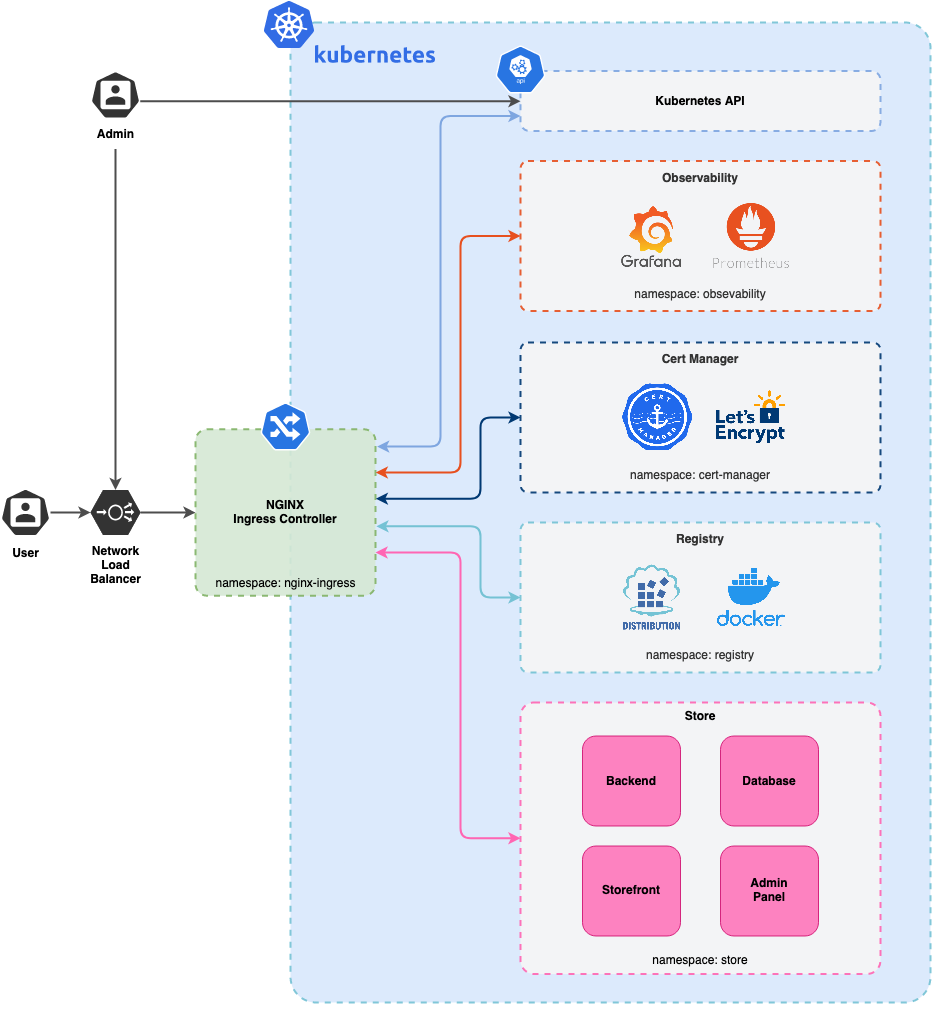
\includegraphics[width=\textwidth]{img/main-infra-model}
    \caption{Model platformy sklepu internetowego tulski}
    \label{fig:platform-model}
\end{figure}

\subsection{Platforma wdrożeniowa}\label{subsec:platforma-wdrozeniowa-kubernetes}

Platformą wdrożeniową dla projektu jest infrastruktura w postaci klastra Kubernetes uruchomionego w chmurze Oracle Cloud Infrastructure.
Klaster składa się z czterech węzłów, każdy wyposażony w 1 procesor Oracle CPU oraz 6 GB pamięci RAM\@.
W skład infrastruktury wchodzi również Network Load Balancer, który dystrybuuje ruch sieciowego pomiędzy węzłami klastra.
Wszystkie elementy infrastruktury zostały zaprojektowanie i wdrożone zgodnie z instrukcjami zawartymi w załączniku~\ref{sec:instrukcja-stworzenia-klastra-kubernetes}.

\subsection{Ingress Controller}\label{subsec:ingress-controller}

Zastosowano NGNIX Ingress Controller, czyli jedną z najpopularniejszych implementacji interfejsu Ingress w środowisku Kubernetes.
Przy użyciu polecenia Helm (zob. listing~\ref{lst:helm-install-ingress-controller}) zainstalowano pakiet \url{oci://ghcr.io/nginxinc/charts/nginx-ingress} w wersji 1.0.2.
NGINX Ingress Controller działa jako DaemonSet, co oznacza uruchomienie jednej instancji na każdym z węzłów klastra.
Dodano integrację z cert-manager do zarządzania certyfikatami TLS\@.

\begin{listing}[H]
    \begin{minted}[xleftmargin=10pt,linenos]{bash}
helm install ingress-nginx \
    --version 1.0.2 \
    --set controller.kind="daemonset" \
    --set controller.hostNetwork=true \
    --set controller.ingressClass.name="public" \
    --set controller.service.create=false \
    --set controller.enableCertManager=true \
    -n ingress-nginx \
    --create-namespace \
    oci://ghcr.io/nginxinc/charts/nginx-ingress
    \end{minted}
    \caption{Polecenie instalujące pakiet oci://ghcr.io/nginxinc/charts/nginx-ingress}
    \label{lst:helm-install-ingress-controller}
\end{listing}

\newpage

\subsection{Konfiguracja DNS}\label{subsec:konfiguracja-dns}

Do konfiguracji DNS domeny tulski.com użyto usług Cloudflare.
Dodano pięć rekordów typu A: admin, api, monitoring, registry i store (zob. rysunek~\ref{fig:dns-tulski-com}).
Każdy z wymienionych rekordów wskazuje na publiczny adres IP Load Balancera i korzysta z funkcji Cloudflare Proxy.

\begin{figure}[H]
    \centering
    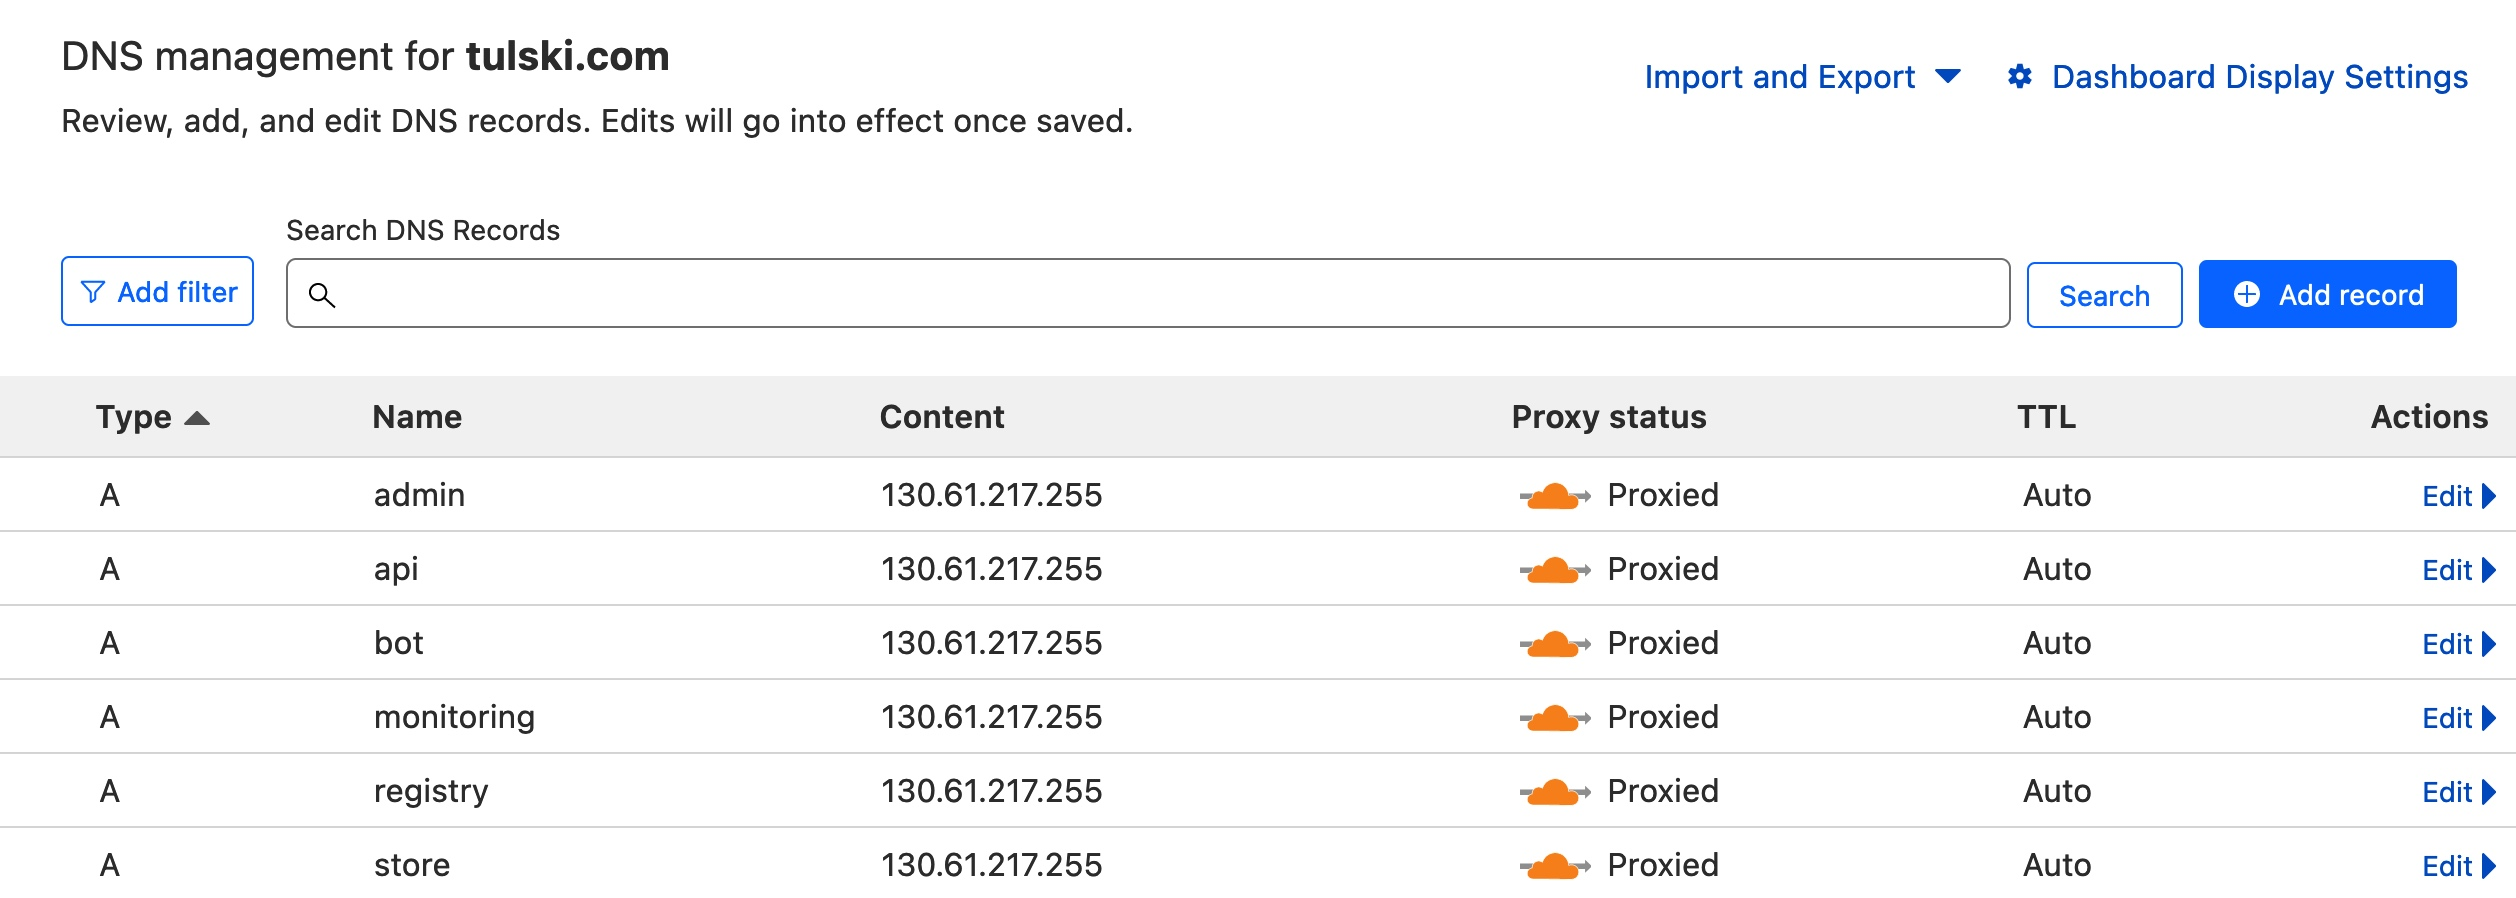
\includegraphics[width=\textwidth]{img/dns-tulski-com}
    \caption{Tabela rekordów DNS dla domeny tulski.com}
    \label{fig:dns-tulski-com}
\end{figure}

\subsection{Monitoring}\label{subsec:monitoring}

\todo{Observability Plane}

\begin{listing}[H]
    \begin{minted}[xleftmargin=10pt,linenos]{bash}
helm install observability \
    -f observability/values.yaml \
    --set "grafana.adminPassword=<adminPassword>" \
    -n observability \
    --create-namespace \
    prometheus-community/kube-prometheus-stack
    \end{minted}
    \caption{Polecenie instalujące pakiet prometheus-community/kube-prometheus-stack}
    \label{lst:helm-install-observability}
\end{listing}

%\begin{figure}[p]
%    \begin{figure}[H]
%        \centering
%        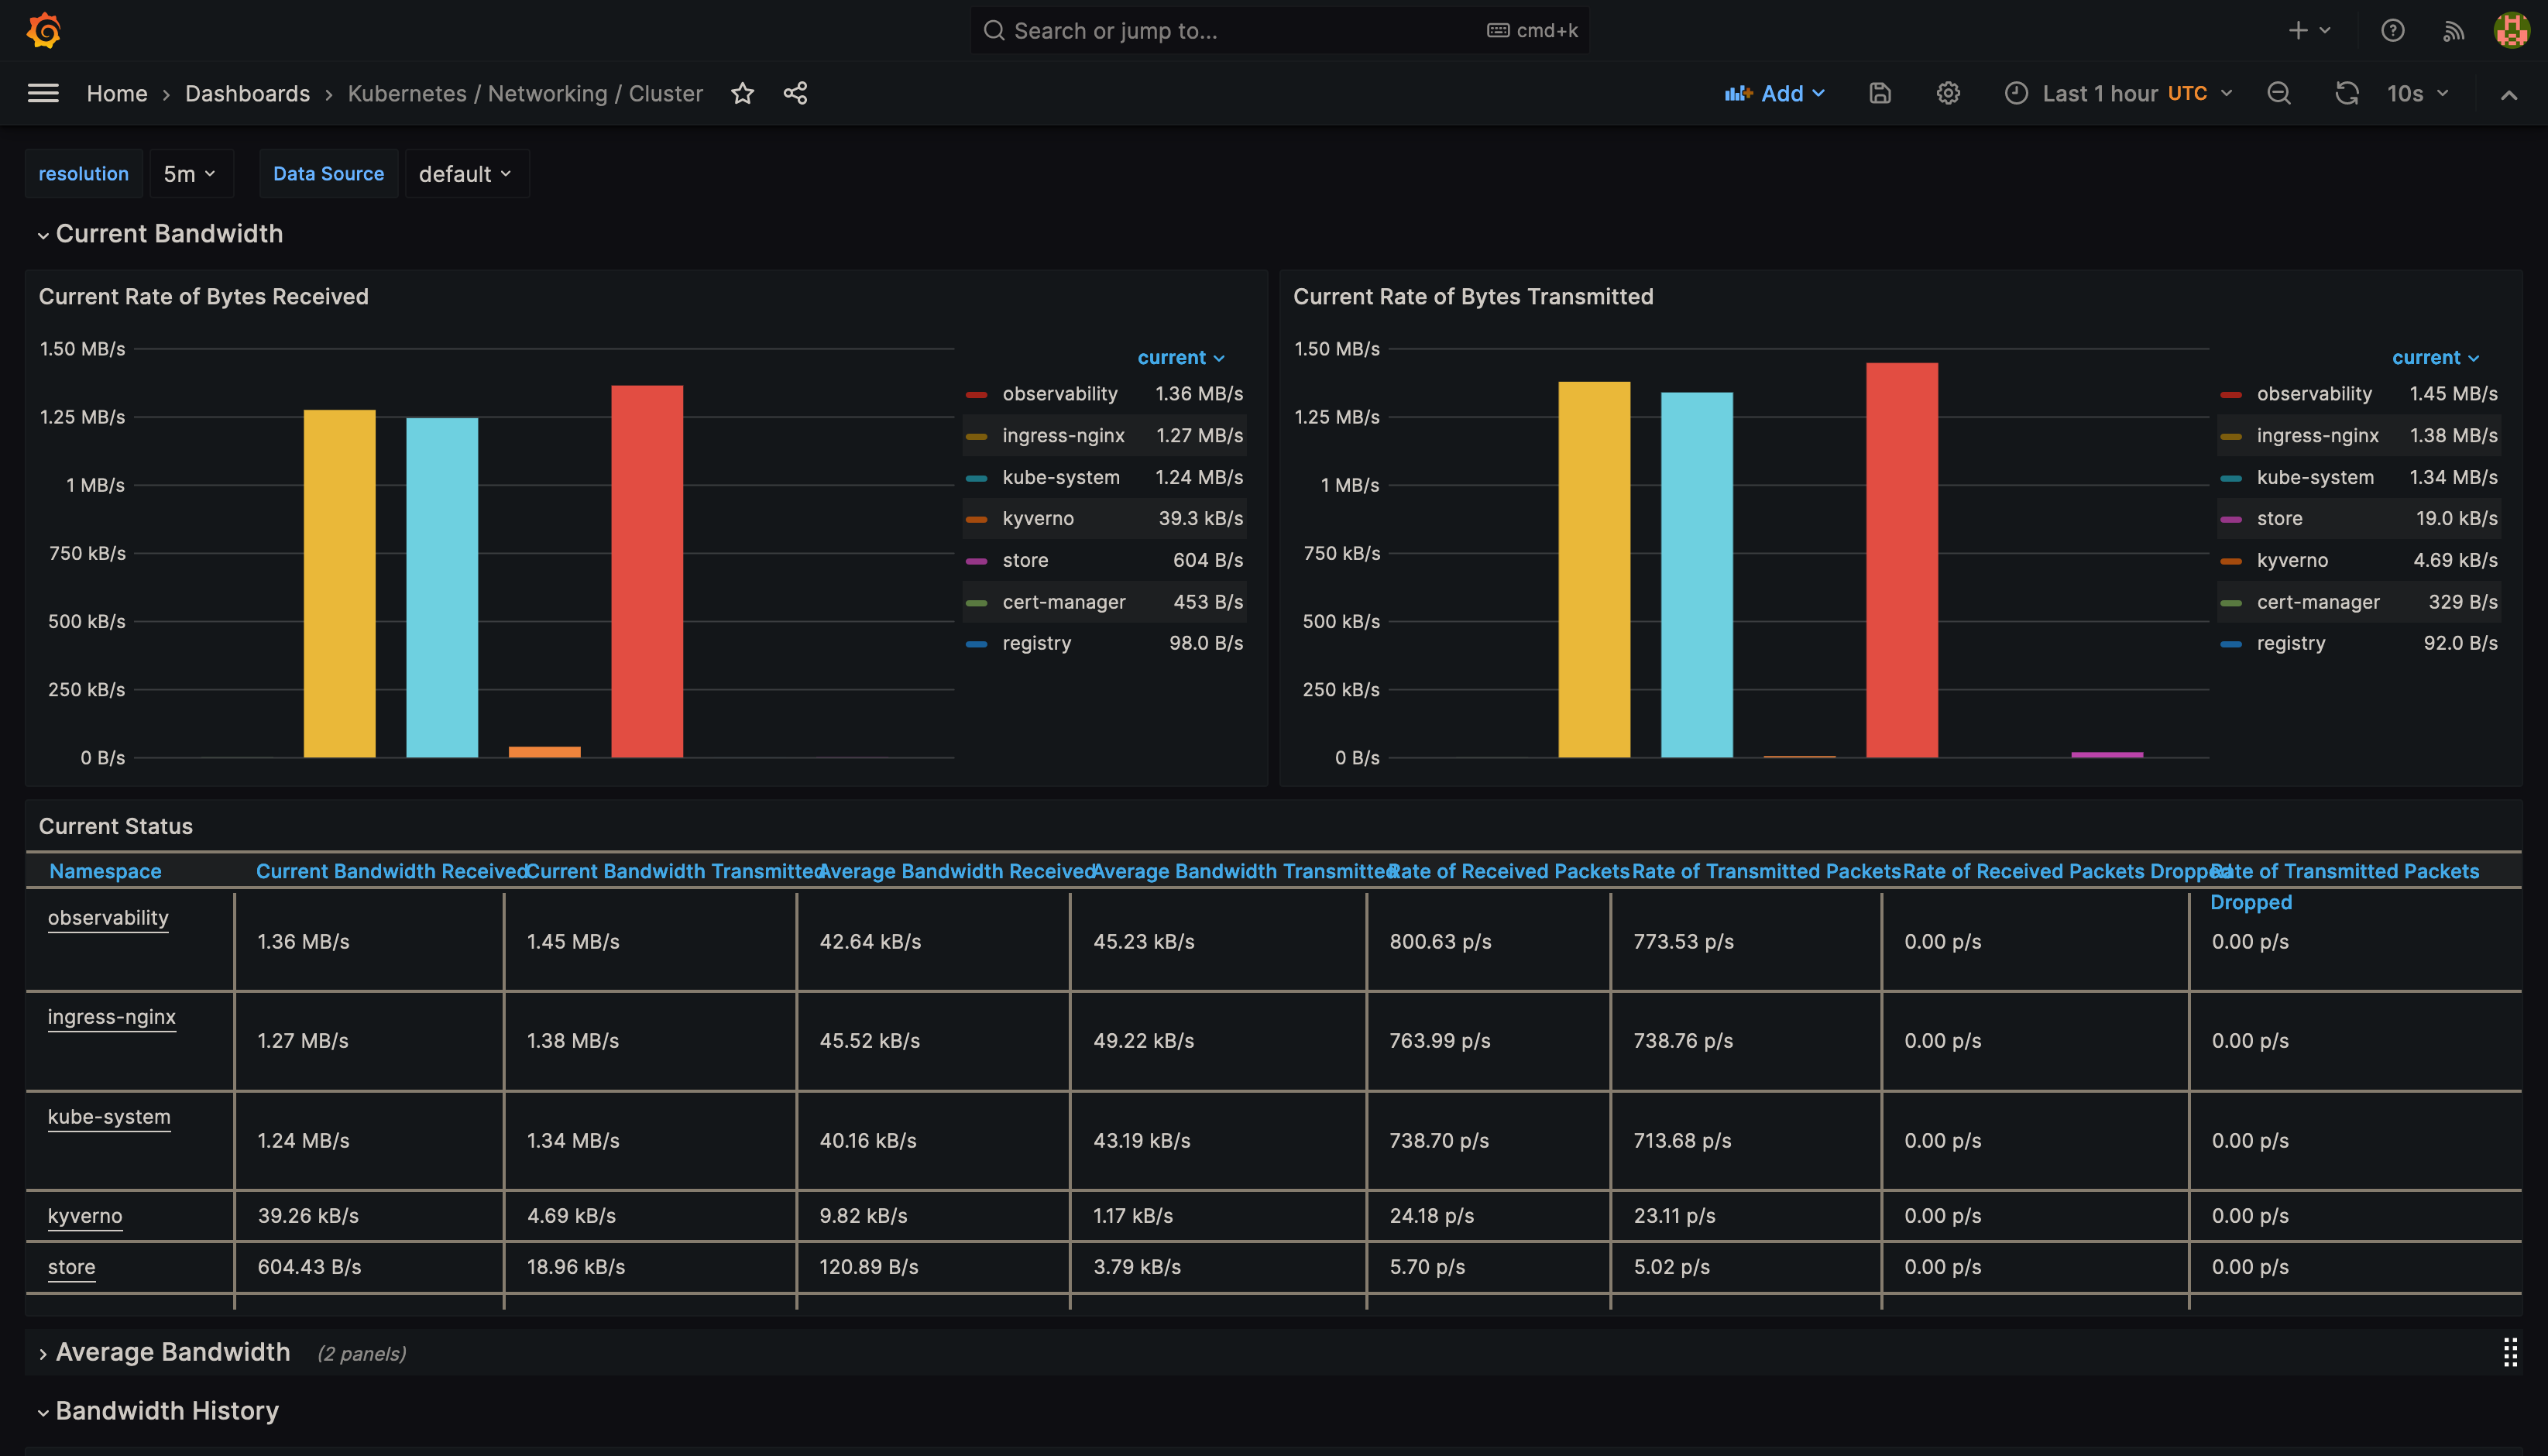
\includegraphics[width=\textwidth]{img/grafana-kubernetes-networking-cluster-dashboard}
%        \caption{Dashboard Kubernetes / Networking / Cluster}
%        \label{fig:grafana-kubernetes-networking-cluster-dashboard}
%    \end{figure}
%
%    \begin{figure}[H]
%        \centering
%        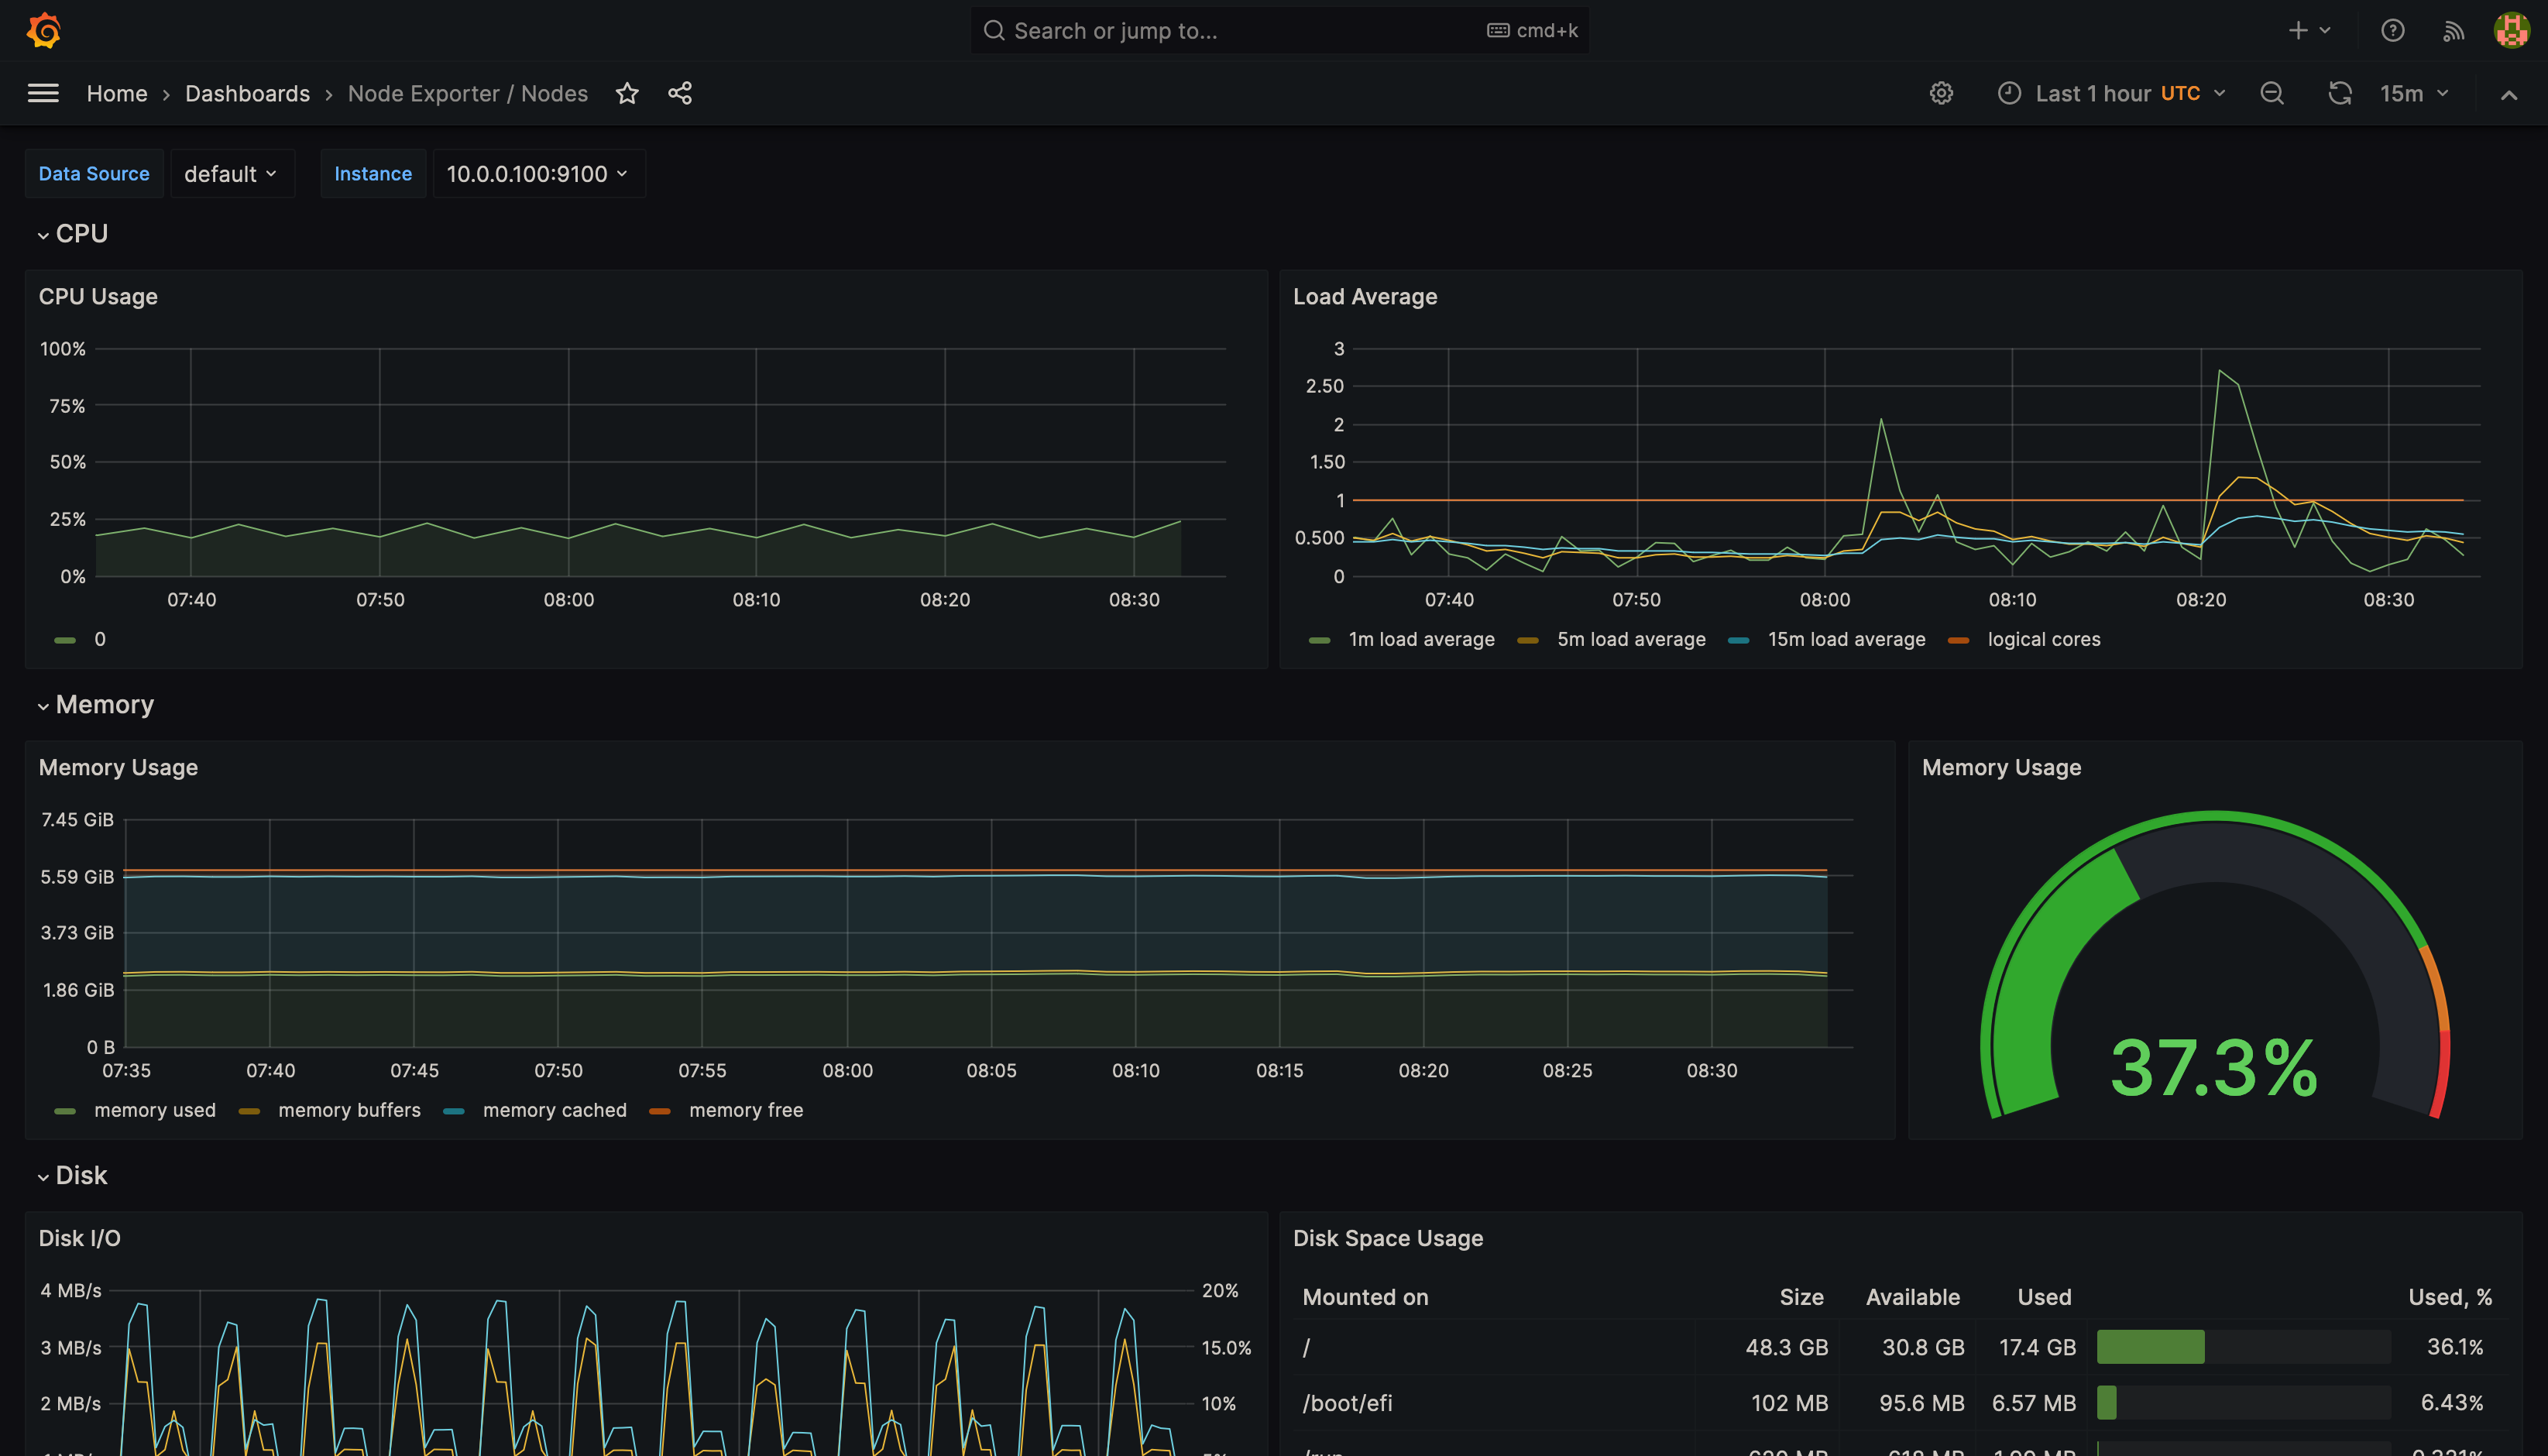
\includegraphics[width=\textwidth]{img/grafana-node-explorer-dashboard}
%        \caption{Dashboard Node Exporter / Nodes}
%        \label{fig:grafana-node-exlorer-dashboard}
%    \end{figure}
%\end{figure}

\subsection{Cert-Manager}\label{subsec:cert-manager-impl}

Wdrożenie cert-manager zostało zrealizowane przy użyciu narzędzia Helm.
Wykorzystano pakiet \url{jetstack/cert-manager} w wersji 1.13.1 (zob. listing~\ref{lst:helm-install-cert-manager}).

\begin{listing}[H]
    \begin{minted}[xleftmargin=10pt,linenos]{bash}
helm install cert-manager \
    --version v1.13.1 \
    --set installCRDs=true \
    --namespace cert-manager \
    --create-namespace \
    jetstack/cert-manager
    \end{minted}
    \caption{Polecenie instalujące pakiet jetstack/cert-manager}
    \label{lst:helm-install-cert-manager}
\end{listing}

\subsection{Docker Registry}\label{subsec:docker-registry}

\todo{Docker Registry}

\subsection{Store}\label{subsec:store}

\subsubsection{Przestrzeń nazw}

Przestrzenią nazw (ang. \emph{namespace}) nazywamy zbiór znaków (nazw) należących do jednego kontekstu.
Ich stosowanie umożliwia lepszą organizację i izolację zasobów, co przyczynia się do podniesienia bezpieczeństwa.
W środowisku Kubernetes przestrzenie nazw umożliwiają segmentację jednego klastra na mniejsze, logicznie wyizolowane jednostki.
Przestrzenie nazw mogą reprezentować środowiska różnych klientów (\emph{tenants}) lub środowiska na różnych poziomach (np. testowe i produkcyjne).

Opisywana platforma posiada przestrzeń nazw o nazwie \url{store}, która zawiera wszystkie elementy niezbędne do działania sklepu internetowego \url{store.tulski.com}.
Przestrzeń \url{store} została stworzona poprzez zaaplikowanie manifestu (zob. listing~\ref{lst:store-namespace}).

\begin{listing}[H]
    \inputminted[xleftmargin=20pt,linenos]{yaml}{code/store-namespace.yaml}
    \caption{Manifest tworzący przestrzeń nazw store}
    \label{lst:store-namespace}
\end{listing}

\subsubsection{Baza danych}\label{subsubsec:baza-danych}

Dane sklepu internetowego są fizycznie przechowywane na dyskach maszyn wirtualnych.
W CLI MicroK8s aktywowano dodatek Hostpath-Storage (zob. listing~\ref{lst:enable-hostpath-storage}), który udostępnia katalog hosta woluminom Kubernetes tj. PersistentVolumes.

\begin{listing}[H]
    \begin{minted}[xleftmargin=10pt,linenos]{bash}
microk8s enable hostpath-storage
    \end{minted}
    \caption{Polecenie aktywujące dodatek Hostpath-Storage}
    \label{lst:enable-hostpath-storage}
\end{listing}

\noindent Bazą danych jest PostgreSQL zainstalowany przy użyciu menadżera pakietów Helm.
Poleceniem \autoref{lst:helm-install-store-db} zainstalowano pakiet \url{bitnamicharts/postgresql} w przestrzeni \url{store}.

\begin{listing}[H]
    \begin{minted}[xleftmargin=10pt,linenos]{bash}
helm install store-db \
    --set auth.postgresPassword="<postgres-password>" \
    --set auth.username="store-db-admin" \
    --set auth.password="<password>" \
    --set auth.database="store" \
    --set metrics.enabled=true \
    --set metrics.serviceMonitor.enabled=true \
    --set metrics.serviceMonitor.namespace="observability" \
    --set metrics.serviceMonitor.labels.release="observability" \
    -n store \
    oci://registry-1.docker.io/bitnamicharts/postgresql
    \end{minted}
    \caption{Polecenie instalujące pakiet bitnamicharts/postgresql}
    \label{lst:helm-install-store-db}
\end{listing}

\subsubsection{Backend}

Backend, w rozumieniu architektury wielowarstwowej, pełni kluczowy element systemu informatycznego.
To warstwa stanowiąca zaplecze technologiczne, która w oparciu na zdefiniowanych regułach biznesowych, odpowiada za obsługę żądań klientów oraz przetwarza dane w sposób zapewniający ich spójność.

Serwer dostarczany przez projekt Medusa nie wymagał żadnych modyfikacji.
Jedynym wymogiem do jego uruchomienia było wybranie i dołączenie odpowiednich wtyczek (ang. \emph{plugins}) odpowiedzialnych za zarządzanie zamówieniami oraz obsługę płatności.
W tym celu zastosowano odpowiednio medusa-fulfillment-manual  i medusa-payment-manual (zob. \autoref{lst:medusa-config-fulfillment-payment}).
Obie te wtyczki można postrzegać jako atrapy (ang. \emph{mocks}), które umożliwiają funkcjonowanie serwera bez konieczności integracji z rzeczywistymi serwisami, takimi jak Stripe czy PayPal.

\begin{listing}[H]
    \begin{minted}[xleftmargin=20pt,linenos]{js}
const plugins = [
    `medusa-fulfillment-manual`,
    `medusa-payment-manual`,
    // ...
];
    \end{minted}
    \caption{Konfiguracja pluginów medusa-fulfillment-manual i medusa-payment-manual}
    \label{lst:medusa-config-fulfillment-payment}
\end{listing}

Aby backend mógł zostać uruchomiony w środowisku Kubernetes, koniecznie było jego skonteneryzowania.
Proces ten został zrealizowany przy użyciu narzędzia Docker.
W tym celu stworzono plik Dockerfile (zob. listing~\ref{lst:code-dockerfile-backend}), który definiuje wszystkie kroki budowania obrazu kontenera.
Plik Dockerfile rozpoczyna się od określenia obrazu bazowego, czyli \url{node:18-alpine}.
Następnie, w kolejnych etapach \url{deps}, \url{builder} i \url{runner}, są kolejno instalowane zależności NPM, budowany jest kod aplikacji oraz przygotowywane jest środowisko uruchomieniowe serwera.

\begin{listing}[H]
    \inputminted[xleftmargin=20pt,linenos]{docker}{code/Dockerfile.backend}
    \caption{Plik Dockerfile.backend}
    \label{lst:code-dockerfile-backend}
\end{listing}

Backend został zainstalowany i skonfigurowany w środowisku Kubernetes.
Wszystkie komponenty i mechanizmy, które składają się na to wdrożenie, zostały przedstawione na rysunku~\ref{fig:kubernetes-backend}.
Wdrożenie odbywa się przez Deployment, co umożliwia automatyzację i skalowanie aplikacji.
Komunikacja z serwisem odbywa się poprzez NGINX Virtual Server, który szyfruje dane za pomocą certyfikatu TLS wygenerowanego przez Cert-Manager.
Backend korzysta z bazy danych PostgresSQL (zob. \autoref{subsubsec:baza-danych}).
Obserwowalność działania aplikacji zapewnia Prometheus Service Monitor.
Sekrety aplikacji są bezpiecznie zarządzane za pomocą mechanizmów Kubernetes Secrets.

\begin{figure}[H]
    \centering
    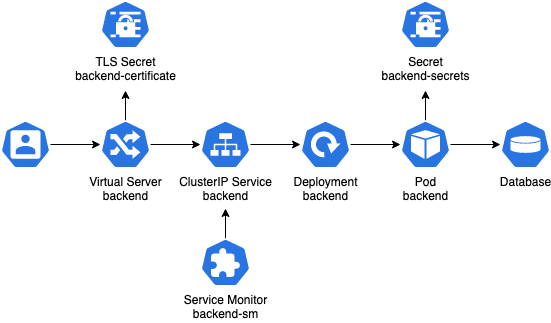
\includegraphics[width=\textwidth]{img/kubernetes-backend}
    \caption{Backend w środowisku Kubernetes}
    \label{fig:kubernetes-backend}
\end{figure}

\subsubsection{Panel administratora}

Panel administratora to kolejny element rozbudowanego ekosystemu Medusa, który jest dostarczany w formie wtyczki (ang. \emph{plugin}).
Panel stanowi graficzny interfejs dla Admin REST API. Jego zastosowanie umożliwia łatwe zarządzanie produktami, zamówieniami oraz ustawieniami sklepu.

Wtyczka panelu administratora, skonfigurowana w plikach serwera backend (zob. listing~\ref{lst:medusajs-admin-plugin}), może być uruchomiona równolegle z backendem, lub jako niezależny serwer.
Zdecydowano się na drugą opcję, ponieważ pozwala ona na niezależne skalowanie obu aplikacji.

\begin{listing}[H]
        \begin{minted}[xleftmargin=20pt,linenos]{js}
const plugins = [
    {
        resolve: "@medusajs/admin",
        options: { /* ... */ },
    },
    // ...
];
        \end{minted}
    \caption{Dołączenie wtyczki @medusajs/admin}
    \label{lst:medusajs-admin-plugin}
\end{listing}

Panel administratora jest budowany do postaci statycznych plików HTML, CSS i JavaScript, które następnie są hostowane przez serwer NGINX (zob. listing~\ref{lst:medusajs-admin-dockerfile}).

\begin{listing}[H]
    \inputminted[xleftmargin=20pt,linenos]{docker}{code/Dockerfile.admin}
    \caption{Plik Dockerfile panelu administratora}
    \label{lst:medusajs-admin-dockerfile}
\end{listing}

Panel administratora w środowisku Kubernetes funkcjonuje jako osobna jednostka wdrożeniowa, niezależna od backendu.
Wykorzystuje NGINX Virtual Server z szyfrowaniem TLS. Certyfikat jest generowany przez Cert-Manager.
Architektura obejmuje service oraz deployment z jednym podem, co przedstawiano na rysunku~\ref{fig:kubernetes-admin}.

\begin{figure}[H]
    \centering
    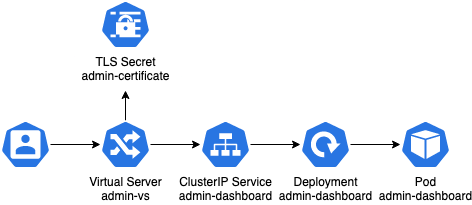
\includegraphics[width=0.9\textwidth]{img/kubernetes-admin-panel}
    \caption{Panel administratora w środowisku Kubernetes}
    \label{fig:kubernetes-admin}
\end{figure}

\subsubsection{Witryna internetowa}

Witryna internetowa, będąca warstwą prezentacyjną systemu, odgrywa kluczową rolę w interakcji z klientem końcowym.
Główny zadaniem tej witryny jest prezentacja oferowanych produktów oraz umożliwienie użytkownikom przeprowadzenia procesu zakupowego.
Projekt Medusa dostarcza szablon witryny sklepu internetowego w formie osobnego projektu o nazwie Storefront.
Storefront, jako graficzny interfejs dla Store REST API, stanowi integralną część reszty systemu Medusa.

Witryna internetowa, analogicznie do części serwerowej oraz panelu administratora, została zintegrowana w strukturze całej platformy poprzez proces skonteneryzowania i wdrożenia w środowisku Kubernetes (zob. rysunek~\ref{fig:kubernetes-storefront}).

\begin{figure}[H]
    \centering
    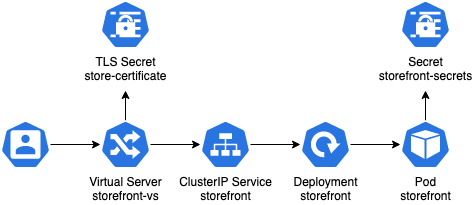
\includegraphics[width=\textwidth]{img/kubernetes-storefront}
    \caption{Witryna internetowa w środowisku Kubernetes}
    \label{fig:kubernetes-storefront}
\end{figure}

Rysunek~\ref{fig:storefront-homepage} przedstawia stronę domową sklepu, akcentując powód jego powstania, czyli niniejszą pracę dyplomową.
Natomiast rysunek~\ref{fig:storefront-products} ilustruje stronę z produktami, ukazując sposób prezentacji asortymentu.
Obie strony razem podkreślają znaczenie estetyki i funkcjonalności w interfejsie użytkownika sklepu internetowego.

\begin{figure}[p]
    \begin{figure}[H]
        \centering
        \fbox{\includegraphics[width=\textwidth]{img/storefront-homepage}}
        \caption{Strona domowa sklepu internetowego}
        \label{fig:storefront-homepage}
    \end{figure}

    \begin{figure}[H]
        \centering
        \fbox{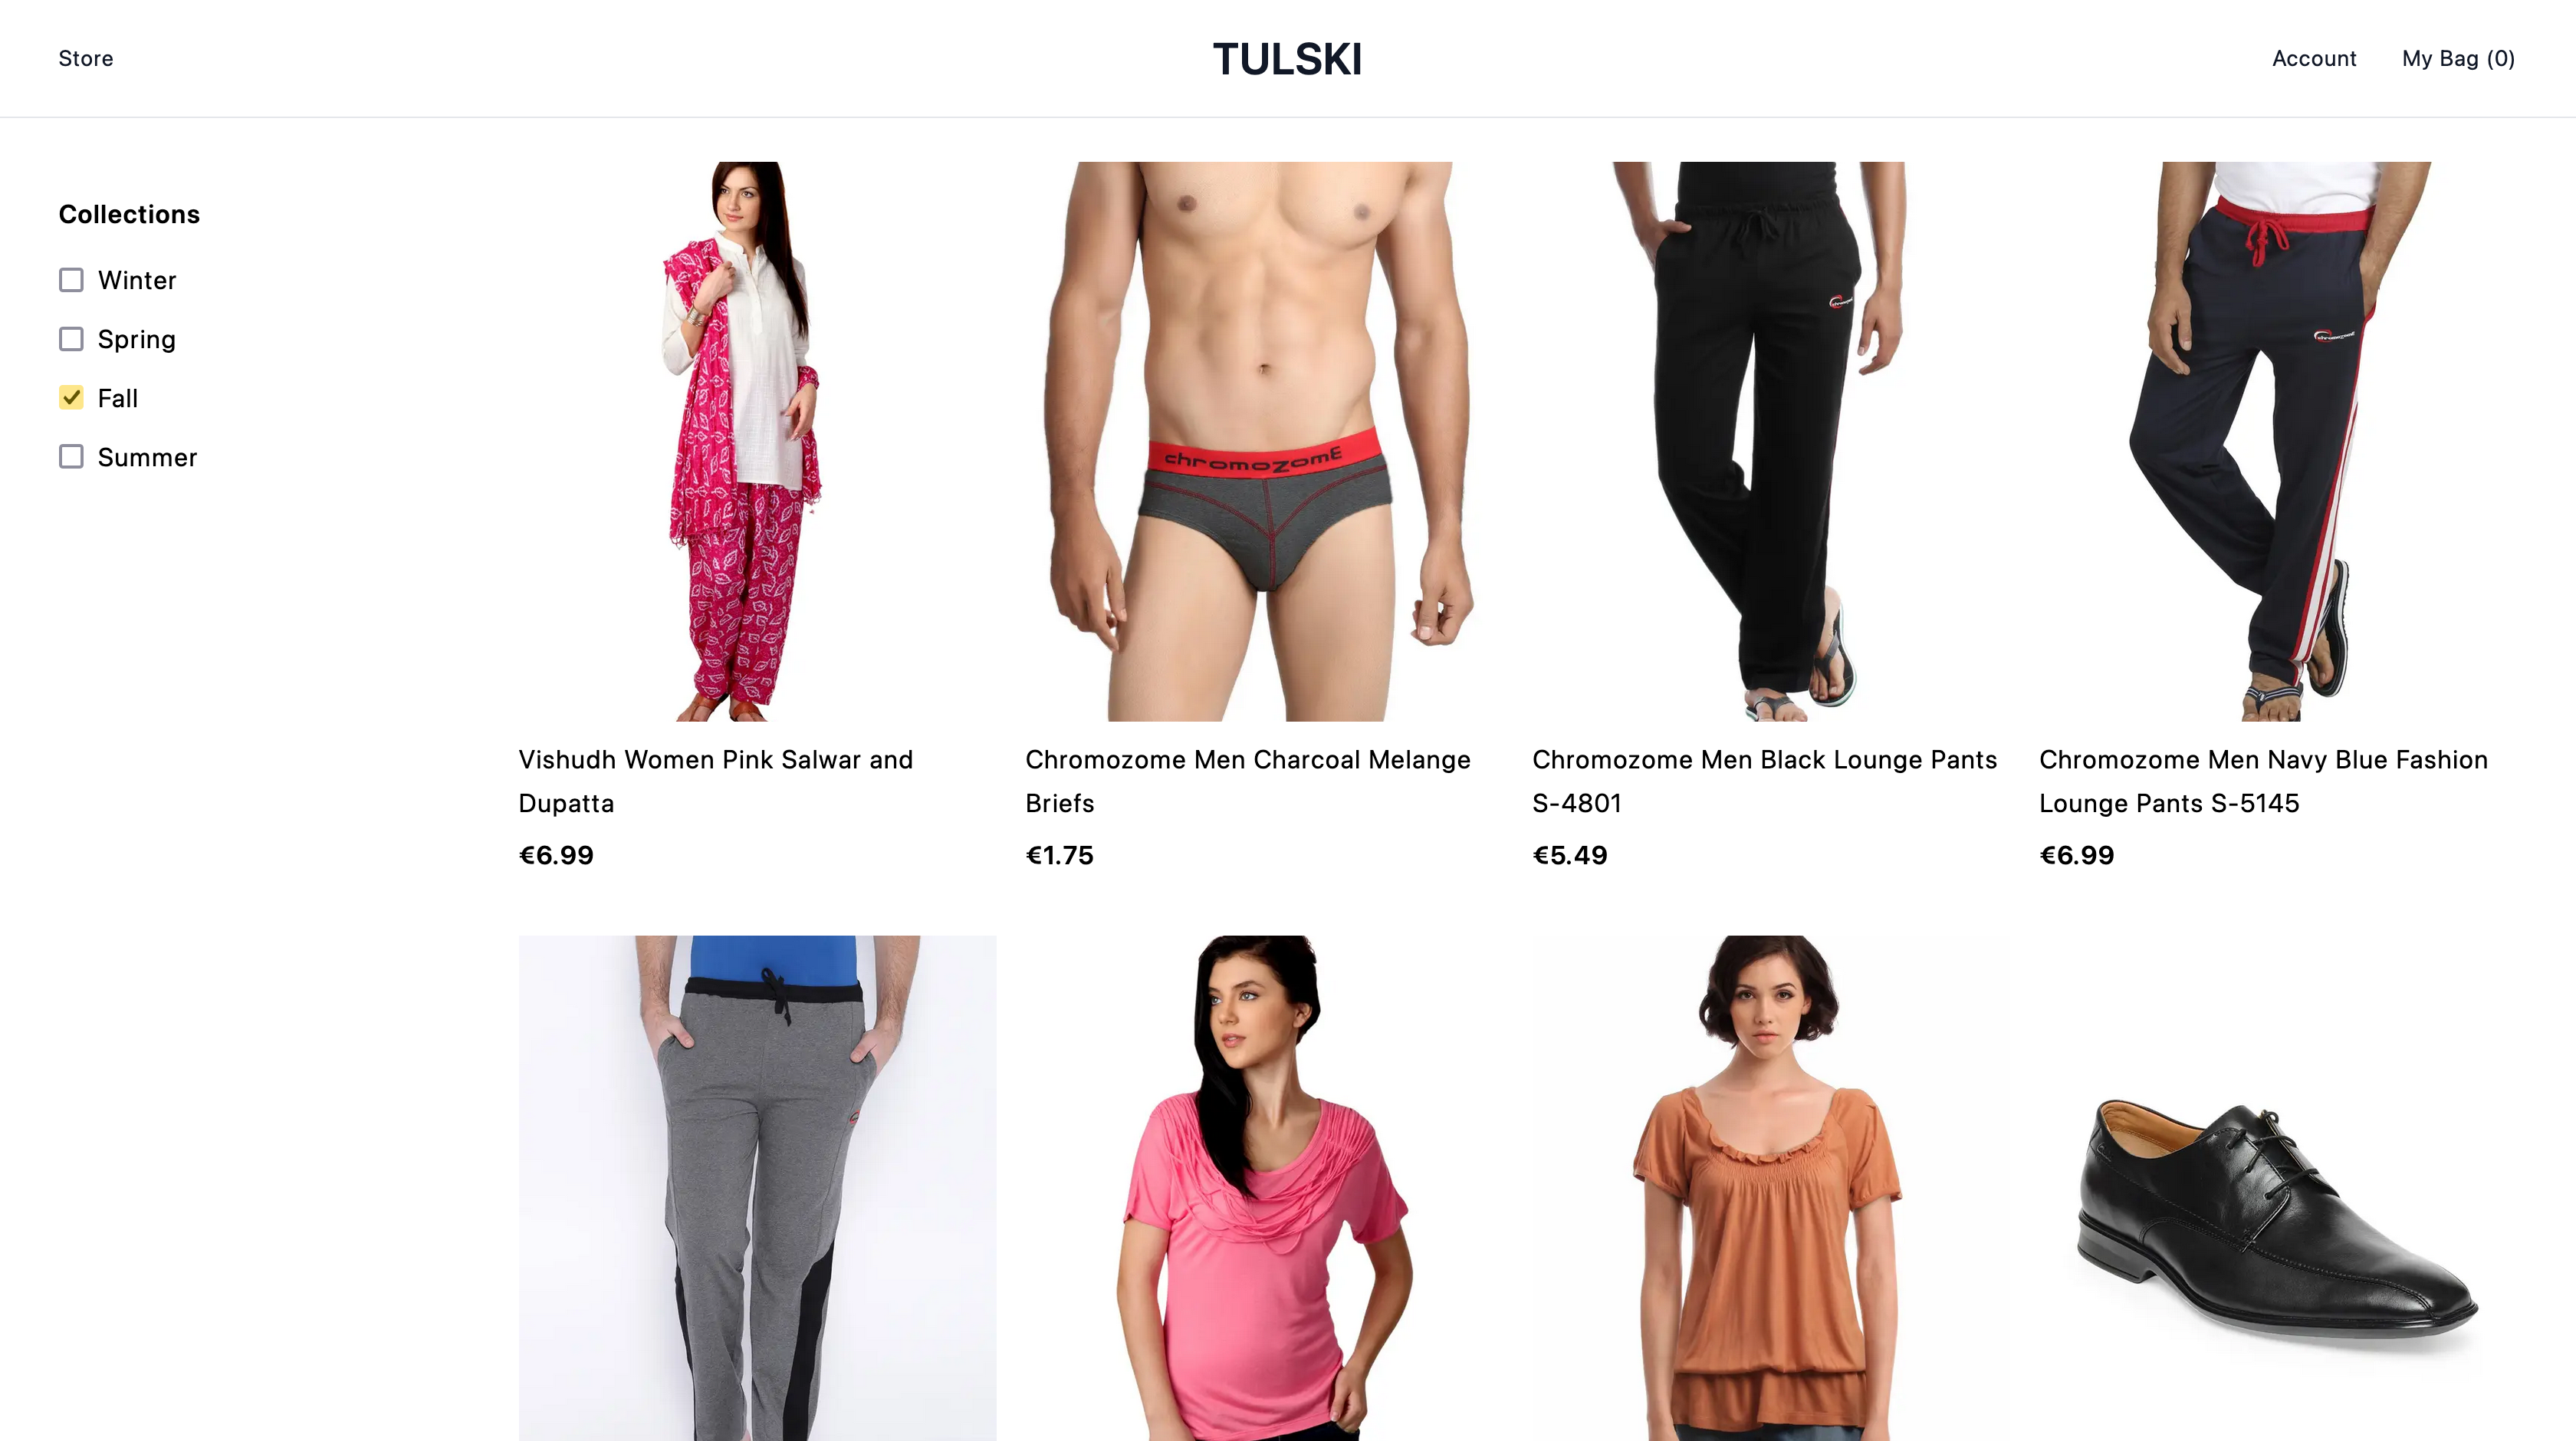
\includegraphics[width=\textwidth]{img/storefront-products}}
        \caption{Strona z produktami sklepu internetowego}
        \label{fig:storefront-products}
    \end{figure}
\end{figure}

\subsubsection{Import produktów}

Sklep internetowy uzupełniono 11440 przykładowymi produktami (zob. listing~\ref{lst:store-count-products}), które pozyskano z zbioru danych~\citetitle*{fashion-dataset}\cite{fashion-dataset} udostępnionego przez~\citeauthor*{fashion-dataset} na platformie Kaggle.

\begin{listing}[H]
    \begin{minted}[xleftmargin=10pt,linenos]{sql}
store=> select count(*) from product;
 count
-------
 11440
(1 row)
    \end{minted}
    \caption{Zapytanie zwracające liczbę wszystkich produktów}
    \label{lst:store-count-products}
\end{listing}


%--------------------------------------------
% Literatura
%--------------------------------------------
\newpage %\cleardoublepage % Zaczynamy od nieparzystej strony
\printbibliography

%--------------------------------------------
% Spisy (opcjonalne)
%--------------------------------------------
\newpage
\pagestyle{plain}

% Wykaz symboli i skrótów.
% Pamiętaj, żeby posortować symbole alfabetycznie
\vspace{0.8cm}
\acronymlist
\acronym{OCPU}{ang. \emph{The Oracle CPU}}
\acronym{OCI}{Oracle Cloud Infrastructure}
\acronym{LB}{Load Balancer}
\acronym{NLB}{Network Load Balancer}

\newpage
\appendix
\appendixpage
\addappheadtotoc

\stopcontents[mainsections]
\startcontents[appendices]
\printcontents[appendices]{l}{1}{\setcounter{tocdepth}{3}}

\newpage

\section{Instrukcja stworzenia klastra Kubernetes}

Ten załącznik stanowi instrukcję stworzenia klastra Kubernetes w chmurze obliczeniowej Oracle Cloud Infrastructure (OCI).
Klaster składa się z czterech węzłów, każdy z nich posiada 1 procesor (Oracle CPU, OCPU) oraz 6 GB pamięci RAM\@.
Zaproponowana infrastruktura obejmuje cztery maszyny wirtualne (c1, c2, c3, c4), load balancer (k8s) oraz sieć wirtualną (subnet-20230313-1902).
Uproszczony i uporządkowany model infrastruktury przedstawiono na rysunku~\ref{fig:infrastructure}.
Wszystkie wymienione elementy zostały wdrożone w ramach darmowego planu \emph{Always Free}.

Wykorzystanie czterech węzłów wraz z load balancerem, oraz odpowiednia konfiguracja, pozwala na zapewnienie wysokiej dostępności (ang. \emph{high availability}).

\begin{figure}[H]
    \centering
    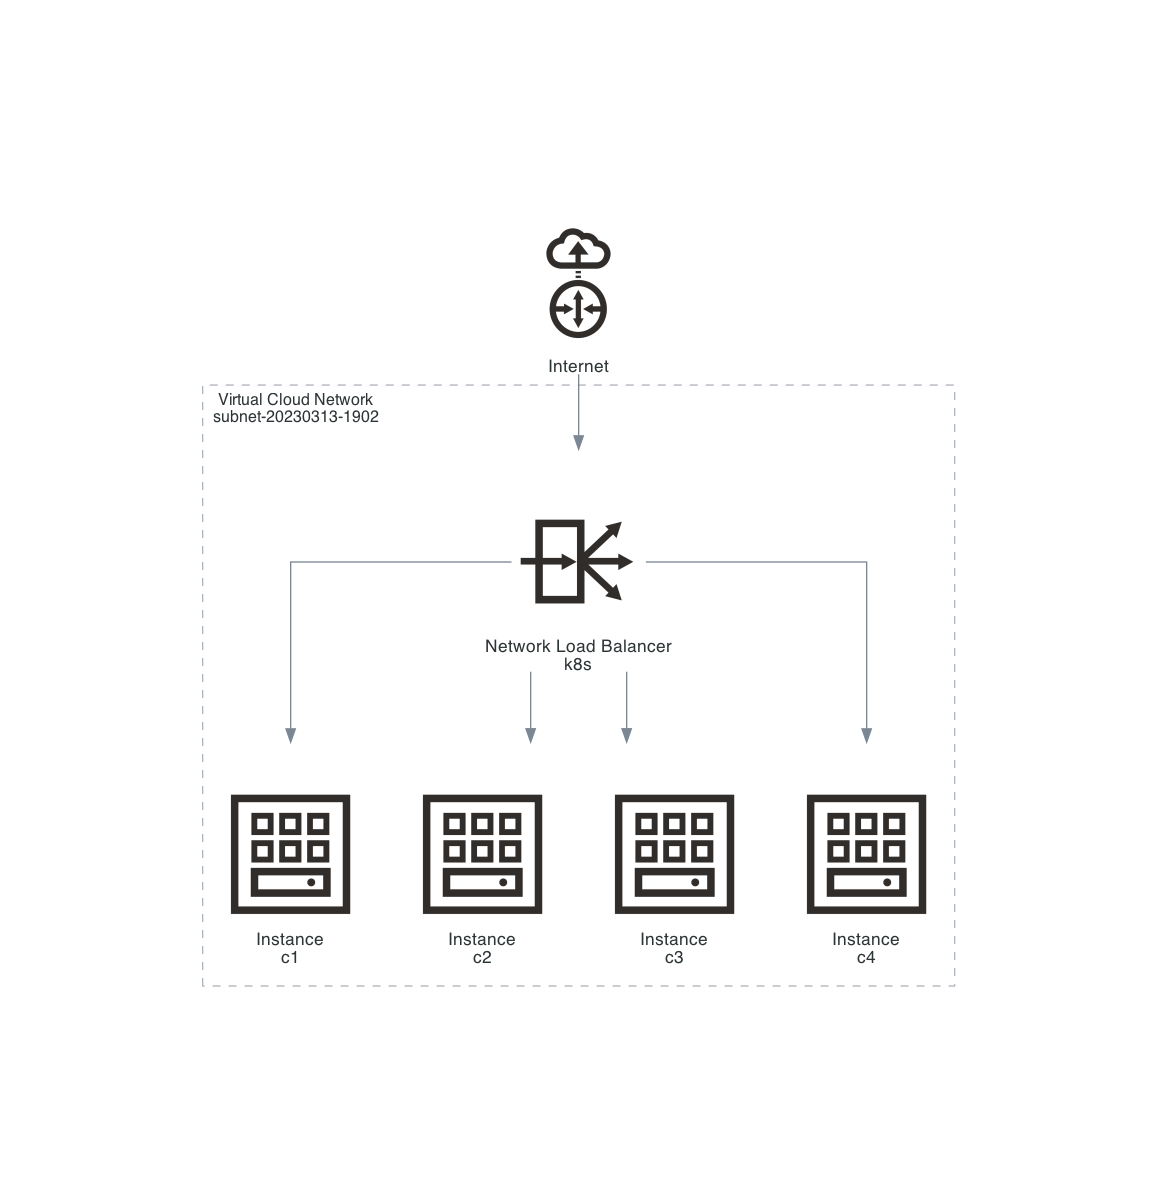
\includegraphics[width=\textwidth]{img/oci-infrastructure}
    \caption{Zaprojektowana infrastruktura}
    \label{fig:infrastructure}
\end{figure}

\subsection{Maszyny wirtualne}

Każdy węzeł klastra został uruchomiony na oddzielnej maszynie wirtualnej (ang. \emph{virtual machine, VM}).
Wszystkie węzły, w formie tabelki, przedstawiono na rysunku~\ref{fig:oci-compute-instances}.

\begin{figure}[H]
    \centering
    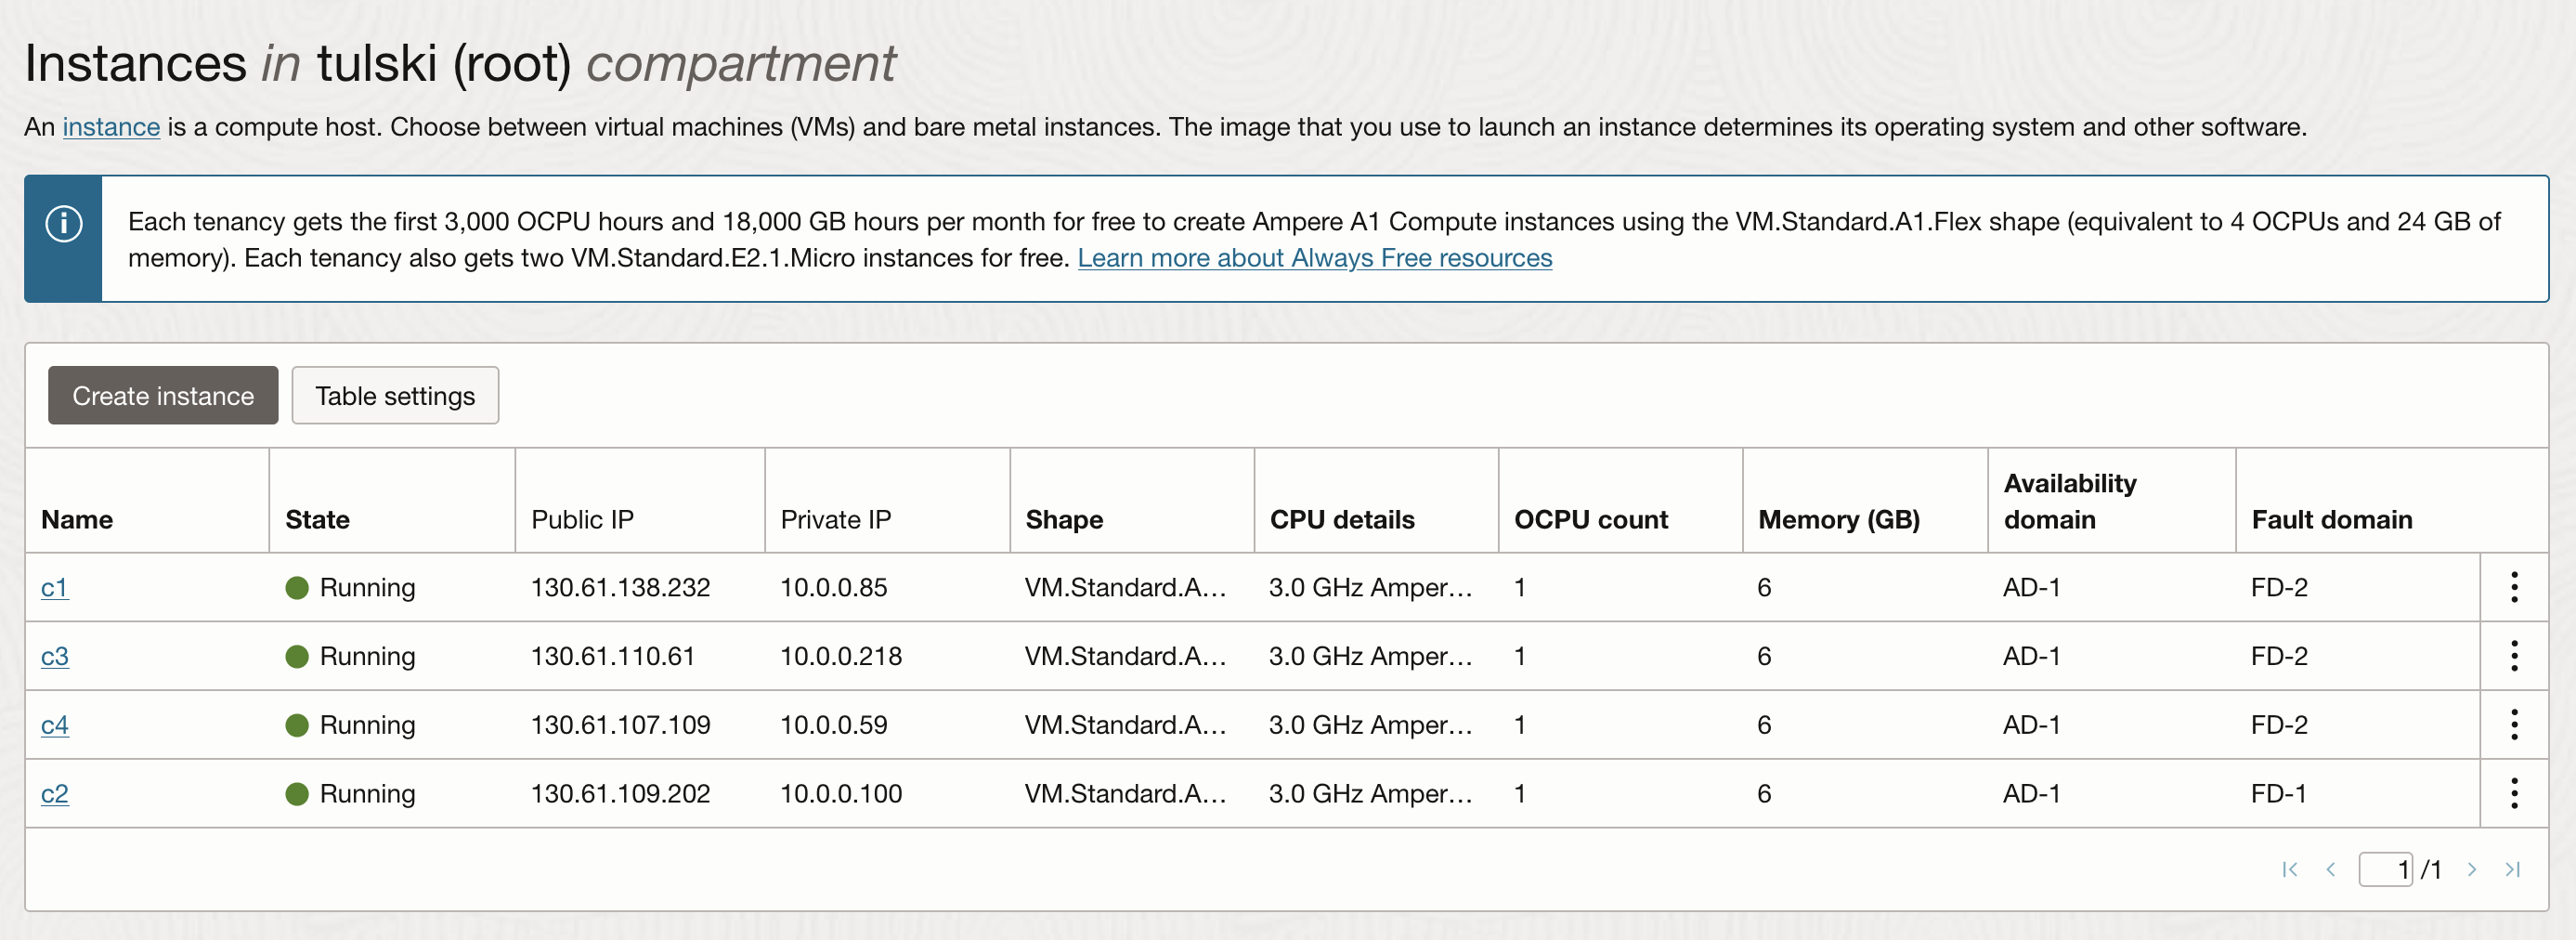
\includegraphics[width=\textwidth]{img/oci-compute-instances}
    \caption{Lista wszystkich maszyn wirtualnych}
    \label{fig:oci-compute-instances}
\end{figure}

\noindent Specyfikacja każdej z maszyn wirtualnych:
\begin{itemize}
    \item Kształt: VM.Standard.A1.Flex (Procesor Arm od Ampere)
    \item Liczba OCPU: 1
    \item Przepustowość sieci: 1 Gbps
    \item Pamięć RAM: 6 GB
    \item Obraz: Canonical Ubuntu 22.04 aarch64 2023.02.15-0
\end{itemize}

\noindent Szczegółową specyfikację jednej z maszyn wirtualnych przedstawiono na rysunku~\ref{fig:oci-instance-details}.

\begin{figure}[H]
    \centering
    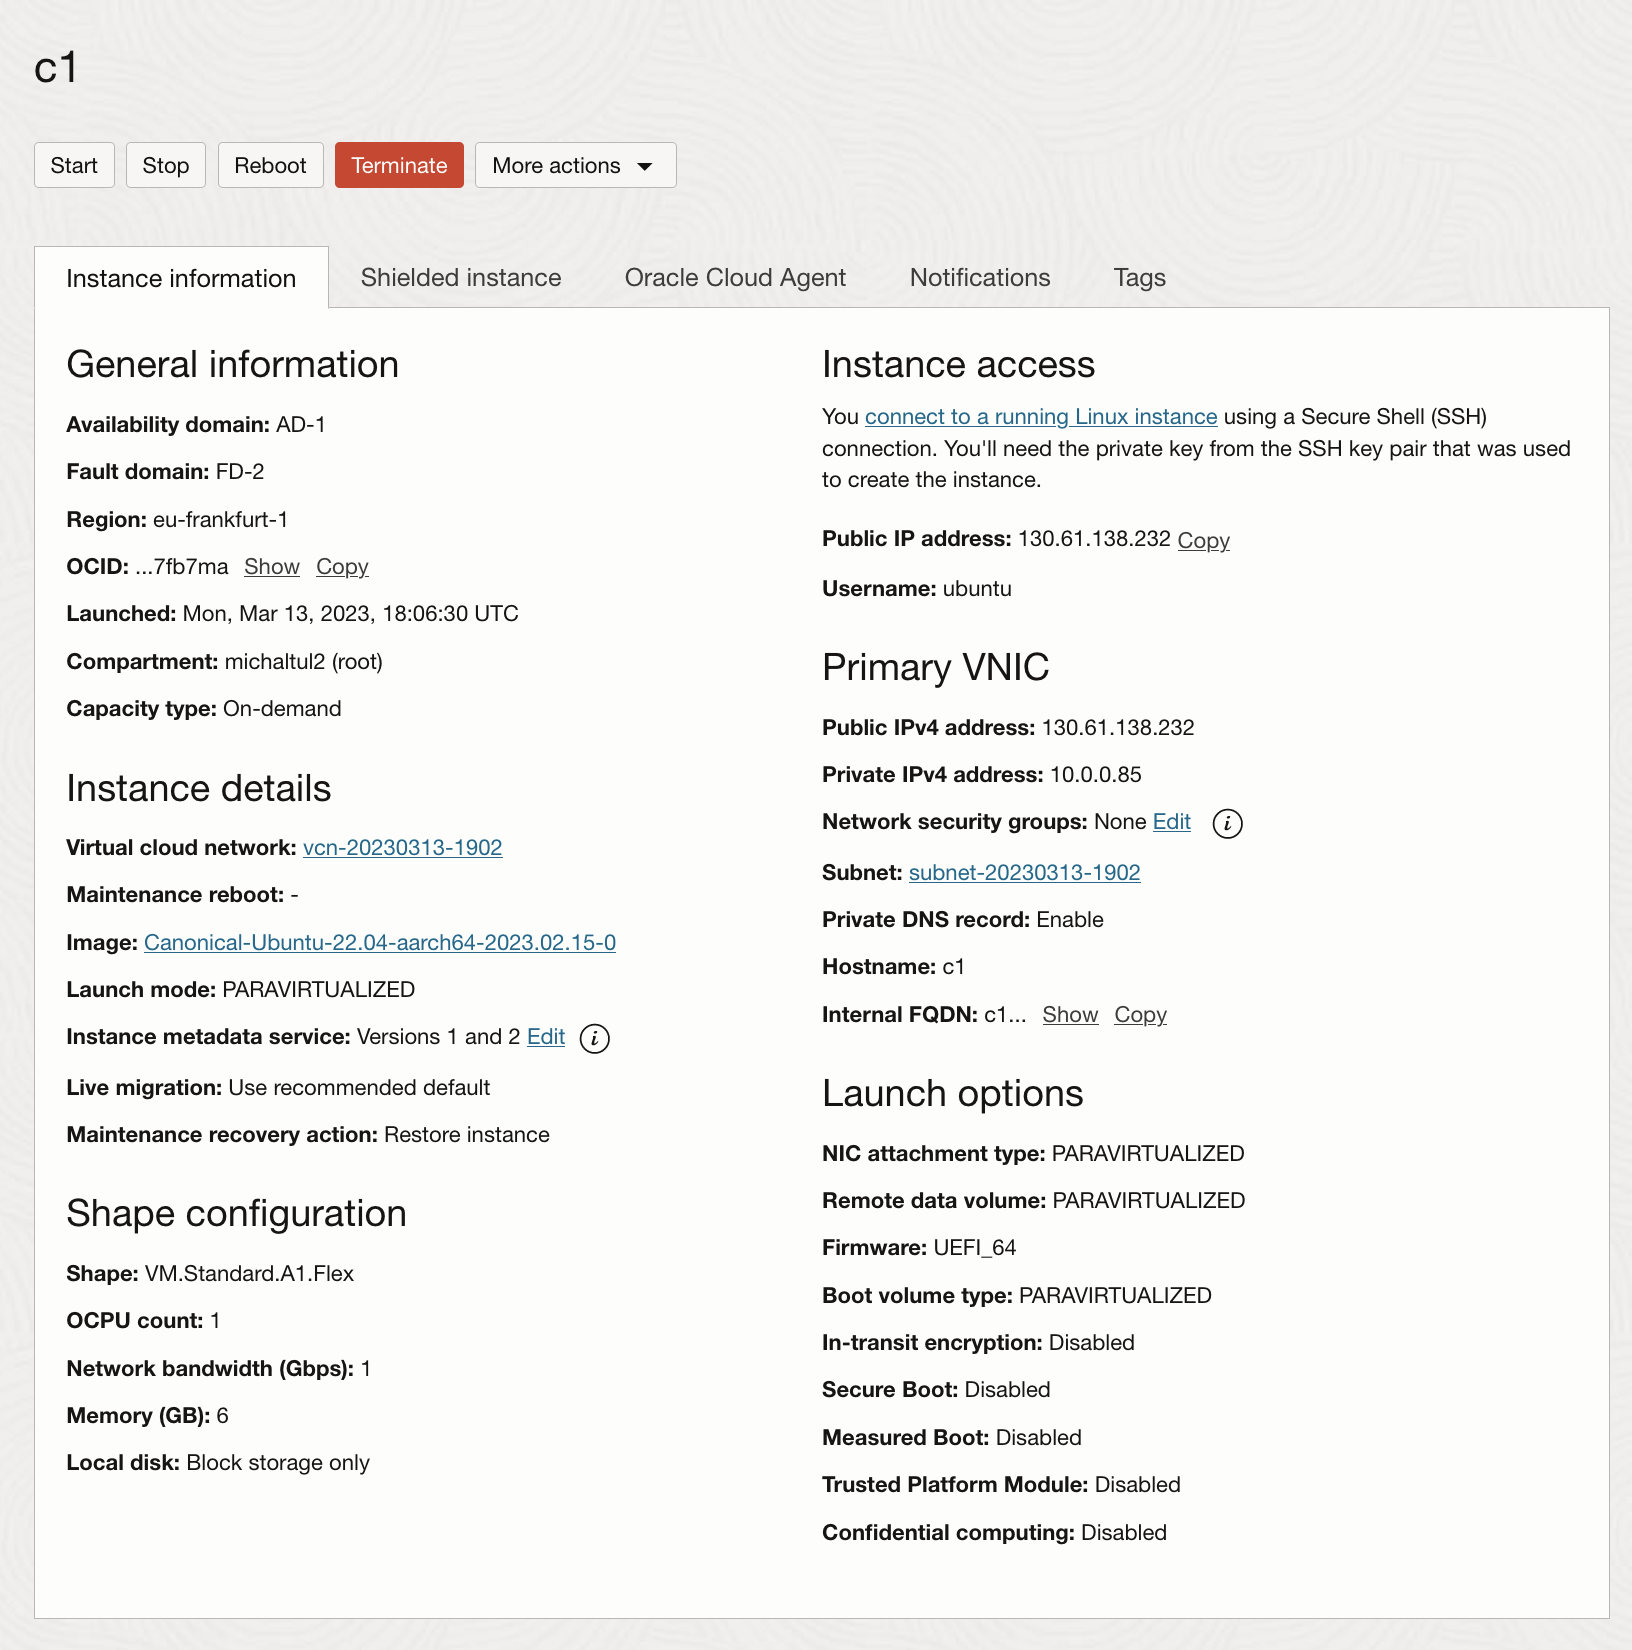
\includegraphics[width=\textwidth]{img/oci-instance-details}
    \caption{Specyfikacja maszyny wirtualnej c1}
    \label{fig:oci-instance-details}
\end{figure}

\subsection{Konfiguracja podsieci}

Wszystkie zasoby znajdują się w jednej wirtualnej podsieci (ang. \emph{virtual cloud network}, VCN) subnet-20230313-1902, która stanowi bezpieczne i izolowane środowisko sieciowe.
Informacje o podsieci przedstawiono na rysunku~\ref{fig:oci-subnet}.

\begin{figure}[H]
    \centering
    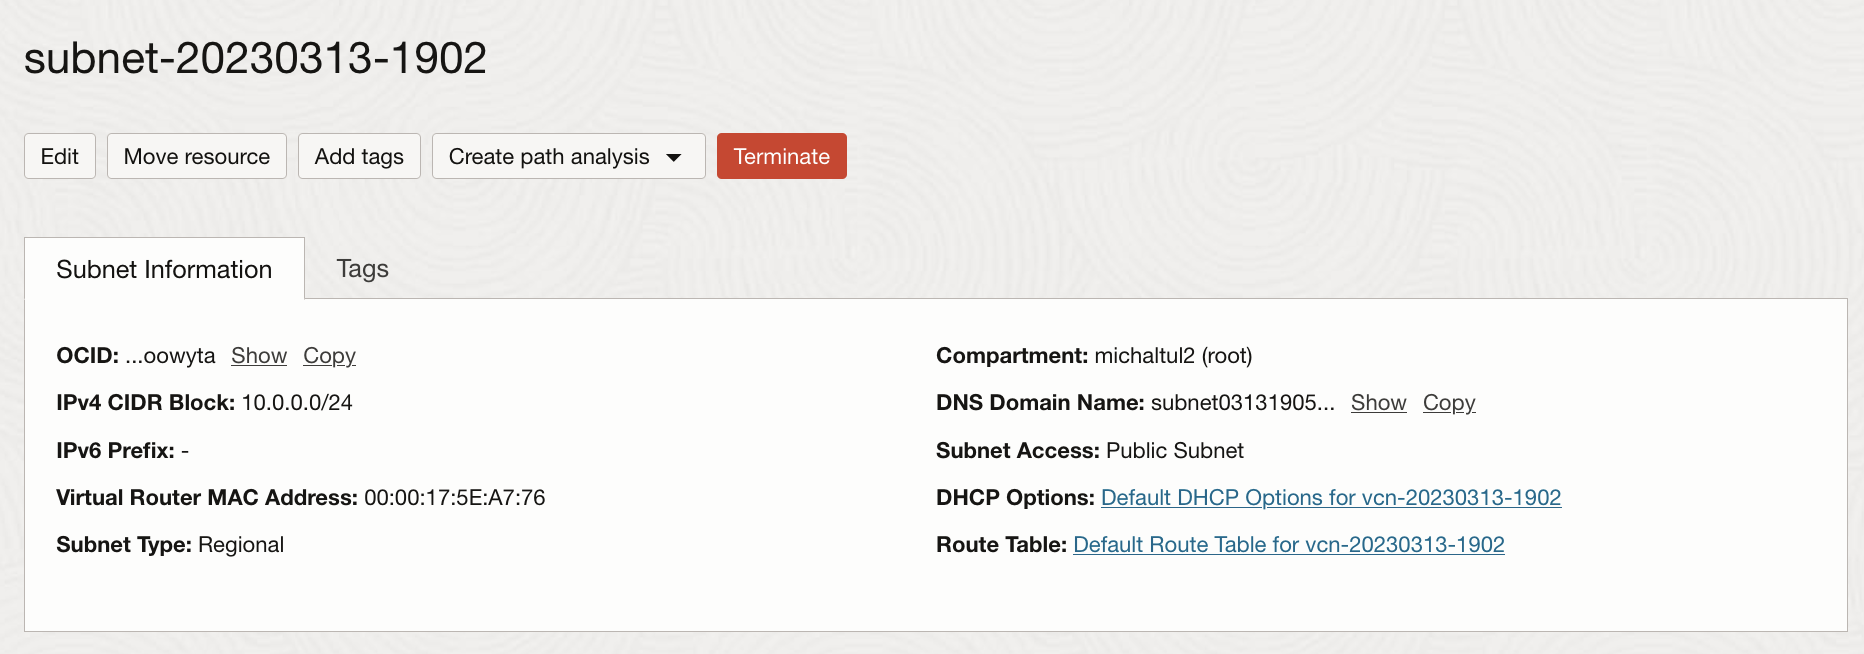
\includegraphics[width=\textwidth]{img/oci-subnet}
    \caption{Podsieć subnet-20230313-1902}
    \label{fig:oci-subnet}
\end{figure}

\noindent Domyślne reguły VCN\cite{oci-security-lists} pozwalają na:
\begin{enumerate}
    \item ruch TCP na porcie usługi SSH (22) z autoryzowanych adresów IP\@,
    \item ruch ICMP typu 3 o kodzie 4 (ang. \emph{Fragmentation Needed and Don't Fragment was Set}) z dowolnego adresu IP,
    \item ruch ICMP typu 3 z wszystkich hostów znajdujących się w danej podsieci,
    \item ruch wychodzący.
\end{enumerate}

\noindent Aby wykorzystać klaster jako platformę wdrożeniową dla aplikacji internetowych, konieczne jest dodanie dwóch dodatkowych reguł.

\begin{enumerate}
    \item Reguła pozwalająca na ruch TCP z dowolnego źródła na porty 80 i 443.
    \item Reguła pozwalająca na cały ruch z adresu IP administratora - wymagana do zdalnego zarządzania klastrem przez Kubernetes API (kubectl).
\end{enumerate}

\noindent Kompletna lista wszystkich reguł sieciowych dla stworzonej podsieci subnet-20230313-1902 została zaprezentowana na rysunku~\ref{fig:oci-subnet-ingress-rules}.

\begin{figure}[H]
    \centering
    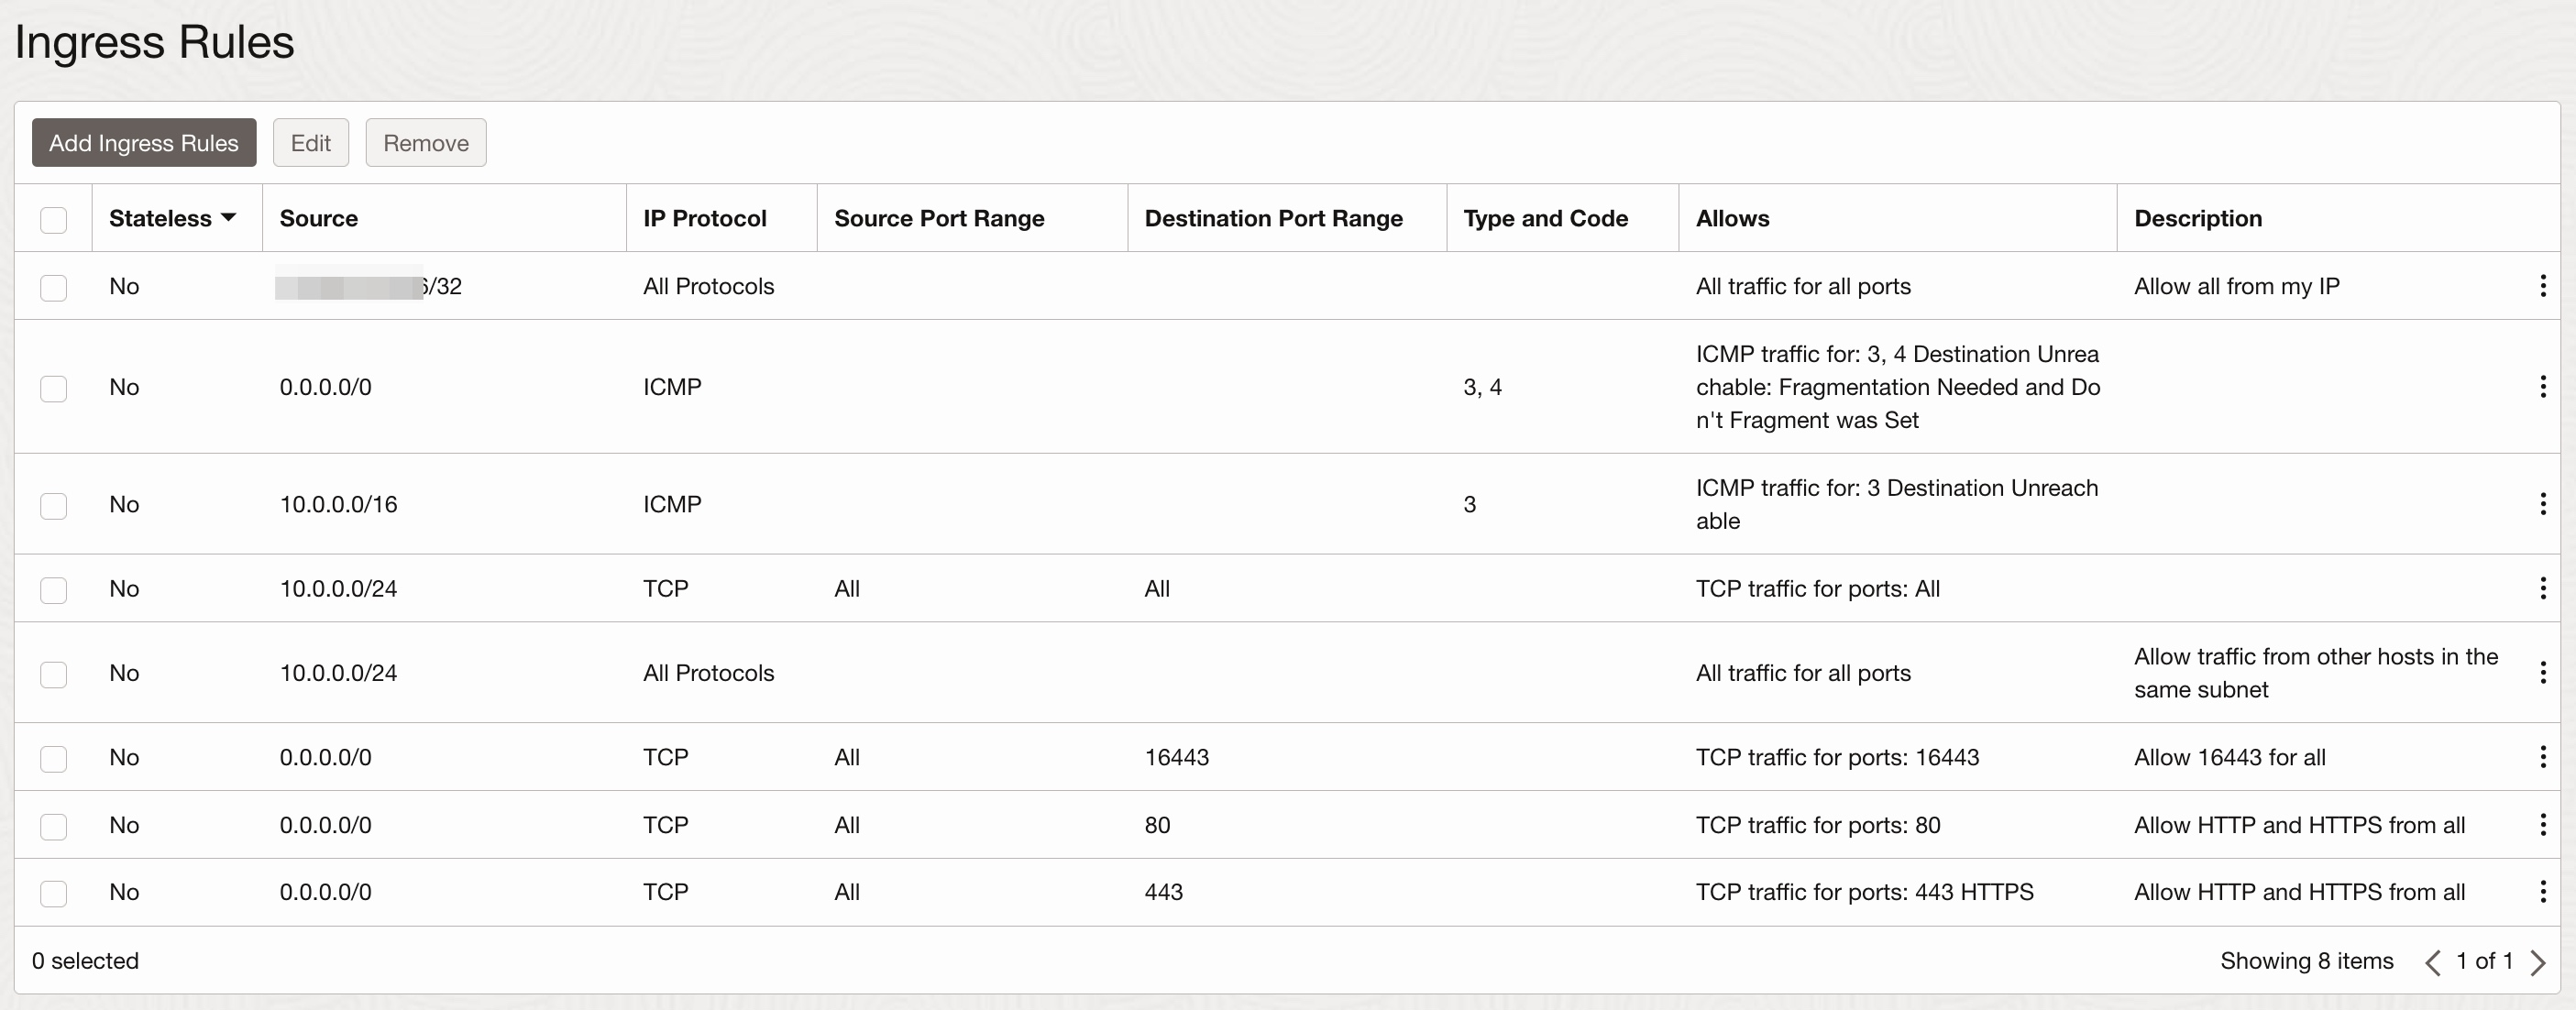
\includegraphics[width=\textwidth]{img/oci-subnet-ingress-rules}
    \caption{Reguły dla ruchu przychodzącego}
    \label{fig:oci-subnet-ingress-rules}
\end{figure}

Zmiany na poziome usług sieciowych OCI są niewystarczające, ponieważ ruch zostanie zablokowany przez domyślne reguły firewalla systemowego maszyn wirtualnych.
Aby osiągnąć oczekiwany rezultat konieczna jest modyfikacja pliku \texttt{/etc/iptables/rules.v4} na każdej z maszyn wirtualnych.

\noindent Należy dodać dwie reguły:

\begin{enumerate}
    \item Reguła zezwalająca na ruch wejściowy pochodzący z publicznego adresu IP administratora.\\
    \mintinline{text}{-I INPUT -s ADMIN_PUBLIC_IP/32 -j ACCEPT}
    \item Reguła pozwalająca na ruch przychodzący z dowolnego adresu w podsieci.\\
    \mintinline{text}{-I INPUT -s 10.0.0.0/24 -j ACCEPT}
\end{enumerate}

\noindent Dodatkowo, konieczne jest usunięcie wpisu, który blokuje wiadomości ICMP (ping):\\
\mintinline{text}{-A FORWARD -j REJECT --reject-with icmp-host-prohibited}

\subsection{Network Load Balancer}

Load Balancer (LB) to technologia, która, podobnie do reverse proxy, ma na celu kierowanie żądań użytkowników do odpowiednich serwerów.
Każdy LB implementuje pewien zestaw reguł i algorytmów, który równomiernie rozkładają ruch na wszystkie serwery w grupie mogące go obsłużyć, tak aby sprostować aktualnemu obciążeniowi.
Dzięki temu zapewnia pryncypium wysokiej dostępności (high availability), niezawodności i skalowalność systemu.
W związku z tym, że Load Balancer ciągle monitoruje aktywność węzłów, jest w stanie szybko wykryć ewentualną awarię i automatycznie przekierować ruch do pozostałych, sprawnych węzłów.
Prostą analogią dla Load Balancera jest policjant stojący na skrzyżowaniu.

Dodatkową zaletą LB jest uproszczenie konfiguracji DNS - wystarczy dodanie jednego rekord typu A z publicznym adresem IP wskazującym na LB\@.
Eliminuje to potrzebę tworzenia osobnych wpisów dla każdego węzła, co komplikowałoby konfigurację i utrudniałoby jej utrzymanie.

Z powodu zapewnienia wysokiej dostępności, równomiernego rozłożenia ruchu, skalowalności i uproszczeniu konfiguracji DNS, jak i wielu innych niewspomnianych korzyści, LB jest kluczowym elementem wielu rozbudowanych systemów.

Jednym z rodzajów Load Balancera jest Network Load Balancer (NLB), który działa na warstwie 3 i 4 modelu OSI wykorzystując protokoły TCP, UDP i ICMP\@.
NLB przekazuje pakiety do i z serwera nadrzędnego na podstawie informacji na poziomie IP, portu i protokołu bez sprawdzania pakietów.

Utworzony Network Load Balancer k8s znajduje się w wcześniej stworzonej podsieci subnet-20230313-1902.

\autoref{fig:oci-network-load-balancer-k8s} przedstawia informacje o wdrożonym NLB k8s.

\begin{figure}[H]
    \centering
    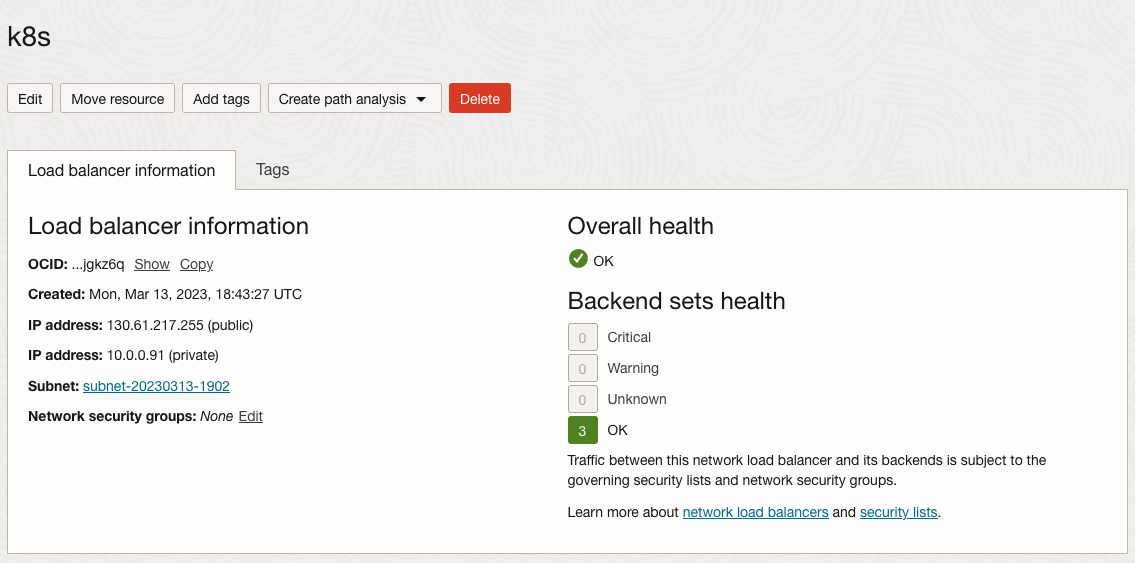
\includegraphics[width=\textwidth]{img/oci-network-load-balancer-k8s}
    \caption{Informacje o NLB k8s}
    \label{fig:oci-network-load-balancer-k8s}
\end{figure}

NLB k8s został skonfigurowany tak aby działał dla ruchu HTTP (port 80), HTTPS (port 443) oraz Kubernetes API (port 16443).
Dla każdego z rodzajów ruchu został utworzony Backend Set (zob. \autoref{fig:oci-network-load-balancer-k8s-backend-sets}) oraz Listener (zob. \autoref{fig:oci-network-load-balancer-k8s-listeners}).

\begin{figure}[H]
    \centering
    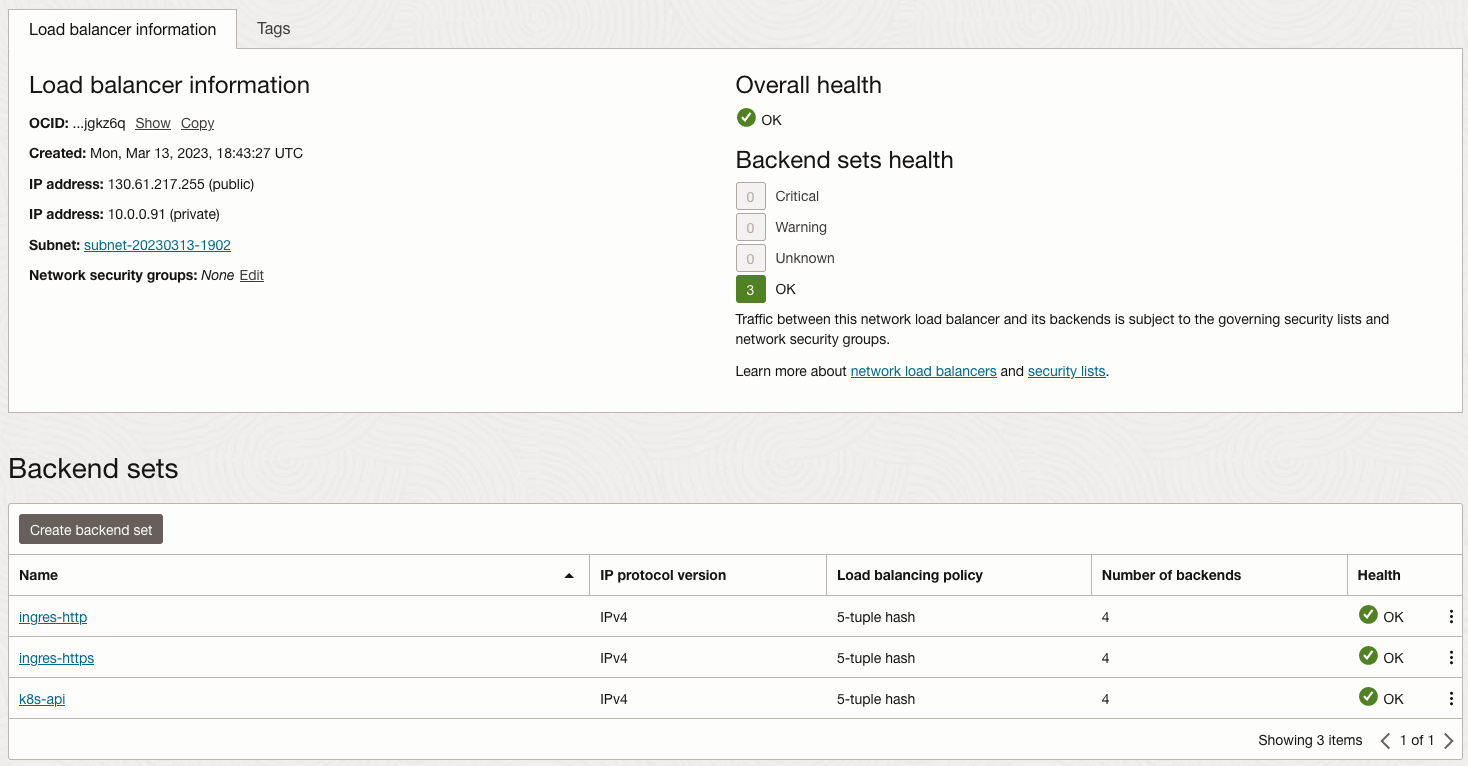
\includegraphics[width=\textwidth]{img/oci-network-load-balancer-k8s-backend-sets}
    \caption{Backend Sets stworzonego Network Load Balancera k8s}
    \label{fig:oci-network-load-balancer-k8s-backend-sets}
\end{figure}

\begin{figure}[H]
    \centering
    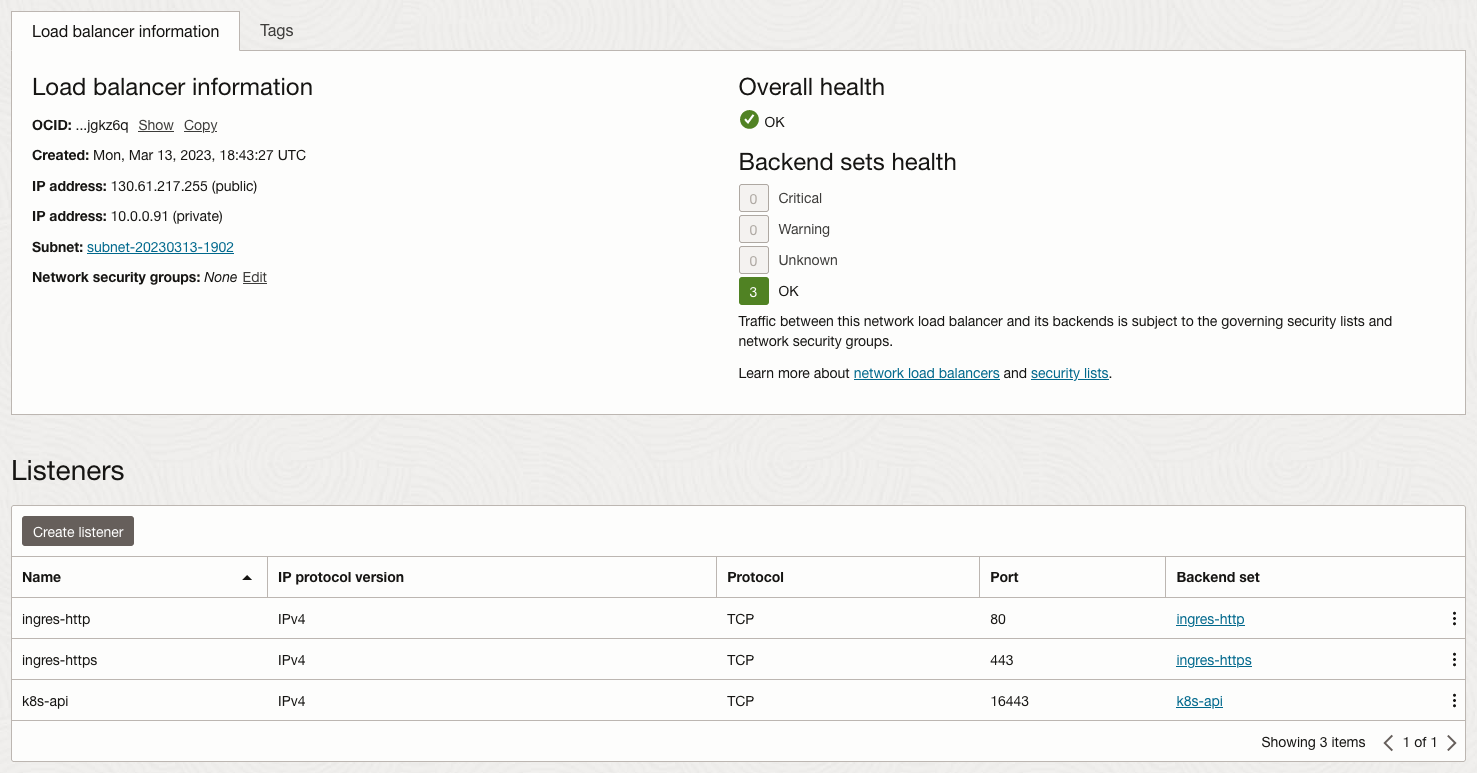
\includegraphics[width=\textwidth]{img/oci-network-load-balancer-k8s-listeners}
    \caption{Listeners stworzonego Network Load Balancera k8s}
    \label{fig:oci-network-load-balancer-k8s-listeners}
\end{figure}

Load Balancer regularnie monitoruje aktywność każdego węzła za pomocą zdefiniowanego testu Health Check.
Dla pierwszych dwóch Backend Sets - \texttt{ingress-http} (zob. \autoref{fig:oci-network-load-balancer-ingress-http-health-check}) oraz \texttt{ingress-https} (zob. \autoref{fig:oci-network-load-balancer-ingress-https-health-check})- test polega na wysłaniu zapytania z użyciem kolejno protokołu HTTP i HTTPS na ścieżkę \url{/}.
Oczekiwaną odpowiedzią serwera jest status 404.

\begin{multicols}{2}
    \begin{figure}[H]
        \centering
        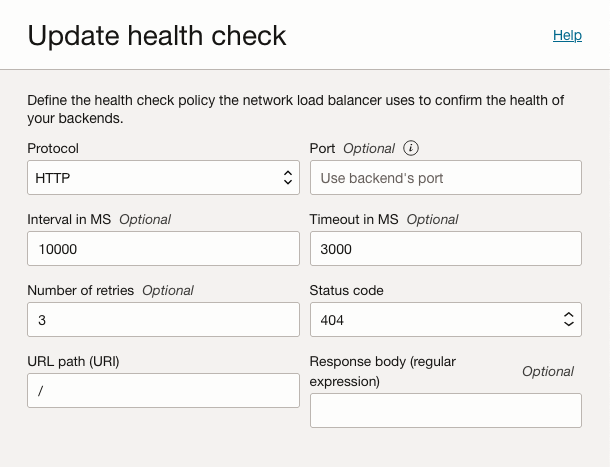
\includegraphics[width=0.5\textwidth]{img/oci-network-load-balancer-ingress-http-health-check}
        \caption{Health Check dla ingress-http}
        \label{fig:oci-network-load-balancer-ingress-http-health-check}
    \end{figure}
    \begin{figure}[H]
        \centering
        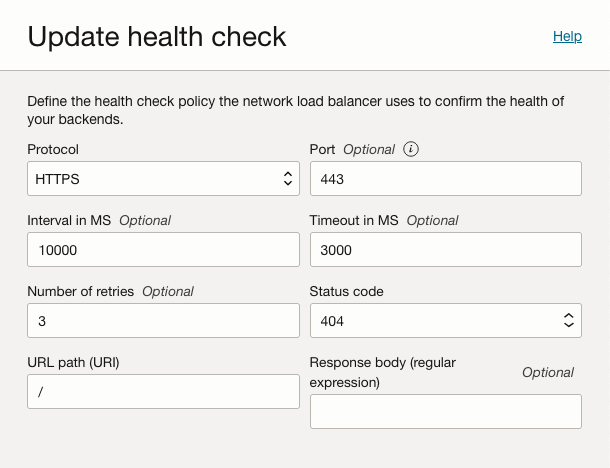
\includegraphics[width=0.5\textwidth]{img/oci-network-load-balancer-ingress-https-health-check}
        \caption{Health Check dla ingress-https}
        \label{fig:oci-network-load-balancer-ingress-https-health-check}
    \end{figure}
\end{multicols}

Ostatni Backend Set, czyli  k8s-api, polega na wysłaniu zapytania protokołem HTTPS na port 16443 do ścieżki \url{/healthz}, gdzie oczekiwaną odpowiedzią serwera jest status 200 (zob. \autoref{fig:oci-network-load-balancer-k8s-api-health-check}).
\begin{figure}[H]
    \centering
    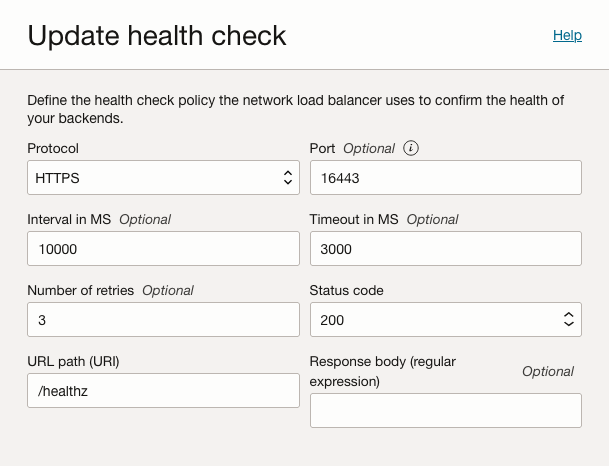
\includegraphics[width=0.7\textwidth]{img/oci-network-load-balancer-k8s-api-health-check}
    \caption{Health Check dla k8s-api}
    \label{fig:oci-network-load-balancer-k8s-api-health-check}
\end{figure}

\subsection{Instalacja Kubernetes}

Klaster wykorzystuje dystrybucję MicroK8s (zob. \autoref{subsec:microk8s}) w wersji 1.23.
Instalację MicroK8s przeprowadzono na każdej z maszyn wirtualnych poleceniem~\autoref{lst:microk8s-install}.

\begin{listing}[H]
    \begin{minted}{bash}
    apt update && \
        apt install docker.io -y && \
        snap install microk8s --classic --channel=1.23/stable
    \end{minted}
    \caption{Polecenie instalacyjne MicroK8s}
    \label{lst:microk8s-install}
\end{listing}

\subsection{Konfiguracja certyfikatów Kubernetes API}

Kubernetes API stanowi kluczowy element systemu z perspektywy cyberbezpieczeństwa.
Jednym z sposobów jego zabezpieczenia jest wymóg szyfrowanej komunikacji HTTPS, opartej na zweryfikowanym certyfikacie.
Domyślne generowane przez MicroK8s certyfikaty pozwalają na połączenia z lokalnych adresów IP (zwykle adresów LAN) oraz komunikację z adresami mDNS (komunikacja w obrębie klastra, z adresów takich jak kubernetes.default lub kubernetes.default.svc.cluster.local).
Aby umożliwić zdalne połączenie z Kubernetes API z internetu, niezbędna jest modyfikacja sekcji alt\_name pliku szablonu Certificate Signing Request (CSR) znajdującego się pod ścieżką \url{ /var/snap/microk8s/current/certs/csr.conf.template}.
Modyfikacja musi zostać wykonana na każdej z maszyn wirtualnych.

\noindent Modyfikacja polega na dodaniu do sekcji alt\_names:
\begin{enumerate}
    \item publicznego adresu IP maszyny wirtualnej,
    \item prywatnego adresu IP maszyny wirtualnej,
    \item publicznego adresu IP load balancera.
\end{enumerate}

\noindent\autoref{lst:domyslna-konfiguracja-alt-names} przedstawia domyślną, niezmienioną sekcję alt\_names.

\begin{listing}[H]
    \begin{minted}{text}
[ alt_names ]
DNS.1 = kubernetes
DNS.2 = kubernetes.default
DNS.3 = kubernetes.default.svc
DNS.4 = kubernetes.default.svc.cluster
DNS.5 = kubernetes.default.svc.cluster.local
IP.1 = 127.0.0.1
IP.2 = 10.152.183.1
    \end{minted}
    \caption{Domyślna sekcja alt\_names maszyny wirtualnej c1}
    \label{lst:domyslna-konfiguracja-alt-names}
\end{listing}

\noindent\autoref{lst:zmodyfikowana-konfiguracja-alt-names} przedstawia odpowiednio zmodyfikowaną sekcję alt\_names.

\begin{listing}[H]
    \begin{minted}{text}
[ alt_names ]
DNS.1 = kubernetes
DNS.2 = kubernetes.default
DNS.3 = kubernetes.default.svc
DNS.4 = kubernetes.default.svc.cluster
DNS.5 = kubernetes.default.svc.cluster.local
IP.1 = 127.0.0.1
IP.2 = 10.152.183.1
IP.100 = 130.61.138.232 # Publiczny adres IP maszyny wirtualnej
IP.110 = 10.0.0.85      # Prywanty adres IP maszyny wirtualnej
IP.120 = 130.61.217.255 # Publiczny adres IP load balancera
    \end{minted}
    \caption{Zmodyfikowana sekcja alt\_names na maszynie wirtualnej c1}
    \label{lst:zmodyfikowana-konfiguracja-alt-names}
\end{listing}

\noindent Po modyfikacji pliku konieczne jest uruchomienie polecenia odświeżającego certyfikaty MicroK8s (zob. \autoref{lst:polecenie-odswiezajace-certyfikaty}) i ponowne uruchomienie maszyny (reboot).

\begin{listing}[H]
    \begin{minted}{bash}
    sudo microk8s refresh-certs
    \end{minted}
    \caption{Polecenie odświeżające certyfikaty MicroK8s}
    \label{lst:polecenie-odswiezajace-certyfikaty}
\end{listing}

\subsection{Formowanie klastra Kubernetes}

\noindent Formowanie klastra w Kubernetes polega na zintegrowaniu węzłów uruchomionych na różnych maszynach wirtualnych, aby wspólnie tworzyły jednolity system.
Poniżej przedstawione są kroki niezbędne do uformowania klastra.

\begin{enumerate}
    \item Określ, która z maszyn wirtualnych będzie pełnić rolę głównego węzła (ang. \emph{master node}). To on będzie koordynować dodawanie kolejnych węzłów do klastra.
    \item Na wyznaczonym głównym węźle wykonaj polecenie \mintinline{bash}{microk8s add-node}.
          Wynikiem będzie polecenie do dołączenia do klastra mające postać:
    \begin{figure}[H]
        \begin{minted}{bash}
    microk8s join <vm_private_ip>:25000/<token>
        \end{minted}
        \label{fig:join-cluster-command}
    \end{figure}
    \item Wykonaj otrzymane w poprzednim kroku polecenie na każdej maszynie wirtualnej, która ma zostać częścią klastra, ale jeszcze w nim nie jest.
    \item Dla każdej kolejnej maszyny, która ma dołączyć do klastra, powtarzaj kroki 2 i 3.
\end{enumerate}

\end{document}
